

%----------------------------------------

\newpage


\section{CybergeoNetworks : a multi-dimensional and spatialized bibliometric}{CybergeoNetworks : une analyse bibliométrique multi-dimensionnelle spatialisée}

\label{app:sec:cybergeonetworks}


\stars


\textit{Cette annexe est le fruit d'une collaboration dans le cadre des 20 ans de la revue Cybergeo : initiée par \noun{D. Pumain} (Université Paris 1) et \noun{A. Banos} (Université Paris 1), une équipe interdisciplinaire composée de \noun{C. Cottineau} (University College London), \noun{P.-O. Chasset} (LISER), \noun{H. Commenges} (Université Paris 1), a mené une analyse par méthodes multiples et complémentaires du corpus de la revue Cybergeo. L'article correspondant est ici traduit et adapté.}


\stars


%----------------------------------------

\bpar{
Bibliometrics have become commonplace and widely used by authors and journal to monitor, evaluate and identify their readership in an ever-increasing publishing scientific world. With this contribution, we aim to move from the near-real time counts to investigate the semantic proximities and evolution of the papers published in the online journal Cybergeo since its creation in 1996. We compare three strategies for building semantic networks, using keywords (self-declared themes), citations (areas of research using the papers published in Cybergeo) and full-texts (themes derived from the words used in writing). We interpret these networks and semantic proximities with respect to their temporal evolution as well as spatial expressions, by considering the countries studied in the papers under inquiry. Finally, we compare the three methods and conclude that their complementarity can help go beyond simple statistics to better understand the epistemological evolution of a scientific community and the readership target of the journal.
}{
La bibliométrie est devenue monnaie courante et largement utilisée par les auteurs et les journaux pour suivre, évaluer et identifier le lectorat dans un contexte de publications toujours accrues. Cette contribution vise à se détacher des comptages en temps réel pour s'intéresser les proximités sémantiques et l'évolution des articles publiés dans le journal en ligne Cybergeo depuis sa création en 1996. Nous comparons trois stratégies pour construire des réseaux sémantiques, en utilisant les mots-clés (thématiques auto-déclarées), les citations (aires de recherche utilisant les articles publiés dans Cybergeo) et les textes complets (thèmes dérivés des mots utilisés dans l'écriture). Nous interprétons ces réseaux et les proximités sémantiques selon leur évolution temporelle ainsi que leur inscription spatiale, em considérant les pays étudiés dans les articles considérés. Enfin, nous comparons les trois méthodes et concluons que leur complémentarité peut contribuer à dépasser les simples statistiques pour mieux comprendre l'évolution épistémologique d'une communauté scientifique et de l'audience visée du journal.
}

%\keywords{Geography of Science, Scientometrics, Bibliometrics, Open Science, Networks, Epistemology}
 


%%%%%%%%%%%%%%%%%%%%%
\subsection{Introduction}{Introduction}
%%%%%%%%%%%%%%%%%%%%%

\bpar{
Since the seminal work of Thomas Kuhn in the early 1960s the development of science studies has been based on three disciplinary pillars: history of science, philosophy of science, sociology of science. In the 1980s political science grew in importance studying the links between knowledge production and knowledge utilisation. This ``political turn'' began with the creation of the journal \textit{Knowledge} in 1979. Since late 1990s, science studies has been affected by a ``spatial turn'' and eventually emerged a geography of science \citep{livingston_spaces_1995,livingston_science_2003,livingston_geography_2005,withers_place_2009}. Our work follows this trend: we propose in this paper a spatialised bibliometrics approach.
}{

}

\bpar{
Faced with the increasing number of articles, journals and channels of publication used by researchers in an open access and digital world, journals need tools to identify their readership and authors need this information to better reach their target audience, using the right keywords, vocabulary and citations. This paper provides a set of complementary digital tools which meet three requirements: 1) to go beyond the usual citation metrics and give semantic and network analytics directly from the scientific contents of the papers; 2) to situate the position of sets of papers according to the semantic fields of their topics; 3) to identify the significant variations in research topics that may be linked with the geographical origin of authors or to the country they choose to analyse. This last point is especially interesting for our first case of study which is a journal of geography.
}{

}
 
 
\bpar{
The 20-year anniversary of the first journal exclusively digital in social science – Cybergeo –, was the occasion to analyse a consistent corpus of over 700 articles published in 7 languages, with respect to the geography of its authorship and readership. We performed a quantitative epistemology analysis of the scientific papers published since 1996 to measure their similarities according three types of textual indicators: their keywords (the way authors advertise their research), their citation network (the way the paper is used by other fields and disciplines), or their full-text (the vocabulary used to write the paper and present the research).
}{

}


\bpar{
These analyses are complementary and shows the evolution of a journal towards emergent themes of research. It also highlights the need for Cybergeo to keep extending its authorship base beyond the French-speaking community, in order to match its ambition of a European Journal of Geography. Our contribution consists in these specific epistemological conclusions, but also in a broader methodological and technical input on handling interactively large-scale heterogeneous scientific corpus. We show how the coupling of complementary views can create a second order knowledge: the spatial embedding of the three classification methods unveils unexpected patterns. Furthermore, the dedicated tool that we designed is available as an open source software, that can be used by journals for a collective scientific reflexivity, but also by institutions and individual scientists for a bottom-up empowerment of Open Science.
}{

}


\bpar{
The rest of the paper is organized as follows: we first review similar initiatives tackling heterogeneous or multidimensional approaches to bibliometrics, and describe the case study we work on. We then develop technical details of the different methods used, and how these are coupled through interactive spatial data exploration ; describe results at the first order (each method) and at the second order (achieved through coupling) ; and finally discuss broader implication for quantitative epistemology and reflexivity for Open Science.
}{

}


%%%%%%%%%%%%%%%%%%%%%
\subsubsection{Bibliographic Context}{Contexte bibliographique}


\bpar{
Studies in bibliometrics having as a main focus the complementarity of different approaches are rather sparse. \cite{2016arXiv160106075O} shows that taking into account citation and discipline data into a multilayer network is useful to understand patterns of interdisciplinarity. \cite{cronin2014beyond} is an attempt of an overview of the complex nature of measuring scientific publications and the intrinsic multidimensional nature of knowledge production. It provides both recent technical contributions with critical approaches. It insists on the ``Janus-faced nature of metrics'', confirming that reducing knowledge production to a few dimensions is not only wrong but also dangerous for science. The geographical dimension of science has been studied by numerous targeted studies, such as \cite{maisonobe2013diffusion} that investigates the diffusion of specific questions and practices in molecular biology across the world.
}{

}



\subsubsection{Cybergeo as a case study}{Cybergeo comme cas d'étude}

\bpar{
Cybergeo was founded in 1996 as a digital-only European journal of geography. Since then, 737 scientific articles have been published (until May 2016) by 1351 authors from 51 countries. These articles have generated 2710 citations altogether over the last twenty years, which corresponds to half the number of other articles cited in Cybergeo (5545). 
}{
Cybergeo a été fondé en 1996 comme une journal européen de Géographie entièrement digital. Depuis, 737 articles scientifiques ont été publiés (jusqu'en mai 2016) par 1351 auteurs de 51 pays. Ces articles sont à l'origine de 2710 citations au total sur les 20 dernières années, ce qui correspond à la moitié des autres articles cités dans Cybergeo (5545).
}

\bpar{
Most contributions come from a French institution (561), although French-speaking countries (35 papers from an author affiliated in Canada, 21 in Switzerland) and neighbouring countries (UK: 23 contributions, Italy: 18) are well represented too (fig. \ref{fig:app:cybergeonetworks:authoring}). The geographical subjects of the articles themselves show a larger diversity, as the world is almost fully covered (fig. \ref{fig:app:cybergeonetworks:authoring}). However, France and neighbouring countries such as Spain and Germany are the main focus of the majority of articles, although the United States are the 5th most studied single country. By linking authors to their geographical subject (fig. \ref{fig:app:cybergeonetworks:who}), we find different patterns:
\begin{itemize}
\item European and North American countries studying each other through Cybergeo articles;
\item American countries being studied by authors affiliated in Europe and North-America;
\item African and Asian countries being studied mainly by Europeans and marginally by Americans and themselves;
\item Russia and Australia being studied by Western authors and studying their own hinterland.
\end{itemize}
}{
La majorité des contributions proviennent d'une institution française (561), bien que des pays francophones (35 articles comprennent un auteur affilié au Canada, 21 en Suisse) et des pays voisins (23 contributions pour le Royaume-Uni, 18 pour l'Italie) soient également bien représentés (Fig.~\ref{fig:app:cybergeonetworks:authoring}). Les sujets géographiques des articles aux-mêmes présentent une plus grande diversité, comme le monde est quasiment entièrement couvert (Fig. \ref{fig:app:cybergeonetworks:authoring}). Toutefois, la France et des pays voisins comme l'Espagne ou l'Allemagne sont le sujet principal de la majorité des articles, bien que les Etats-unis soient le 5ème pays le plus étudié. En reliant les auteurs à leur sujet géographique (Fig.~\ref{fig:app:cybergeonetworks:who}), différentes tendances peuvent être mises en valeur :
\begin{itemize}
	\item Des pays européens et nord-américains s'étudiant mutuellement au travers des articles de Cybergeo;
	\item Les pays d'Amérique sont étudiés par des auteurs affiliés en Europe et Amérique du Nord;
	\item Les pays asiatiques et africains sont principalement étudiés par les européens, et de façon marginale par les américains et eux-mêmes;
	\item La Russie et l'Australie sont étudiés par des auteurs occidentaux et étudient leur propre territoire.
\end{itemize}
}


\bpar{
Finally, the temporal evolution shows an accelerated growth of the number of authors – although the number of articles by 5-year period remains stable –, a spread of geographical coverage – with more articles published about emerging countries and extra-European territories –, along with a growing connexion in citation networks. There is a reinforcing bias towards a French-speaking authorship, revealed by the origin of authors as well as by the share of papers published in French.
}{
Enfin, l'évolution temporelle montre une croissance accélérée du nombre d'auteurs - même si le nombre d'articles sur des périodes de 5 ans reste stable, une extension de la couverture géographique, avec plus d'articles publiés sur les pays émergents et les territoires extra-européens, ainsi que des connexions croissantes dans les réseaux de citation. Il existe un biais de renforcement en faveur d'auteurs francophone, révélé par l'origine des auteurs ainsi que la part des articles publiés en français.
}

%%%%%%%%%%%%%%%%%%%
\begin{figure}%[htbp]
	%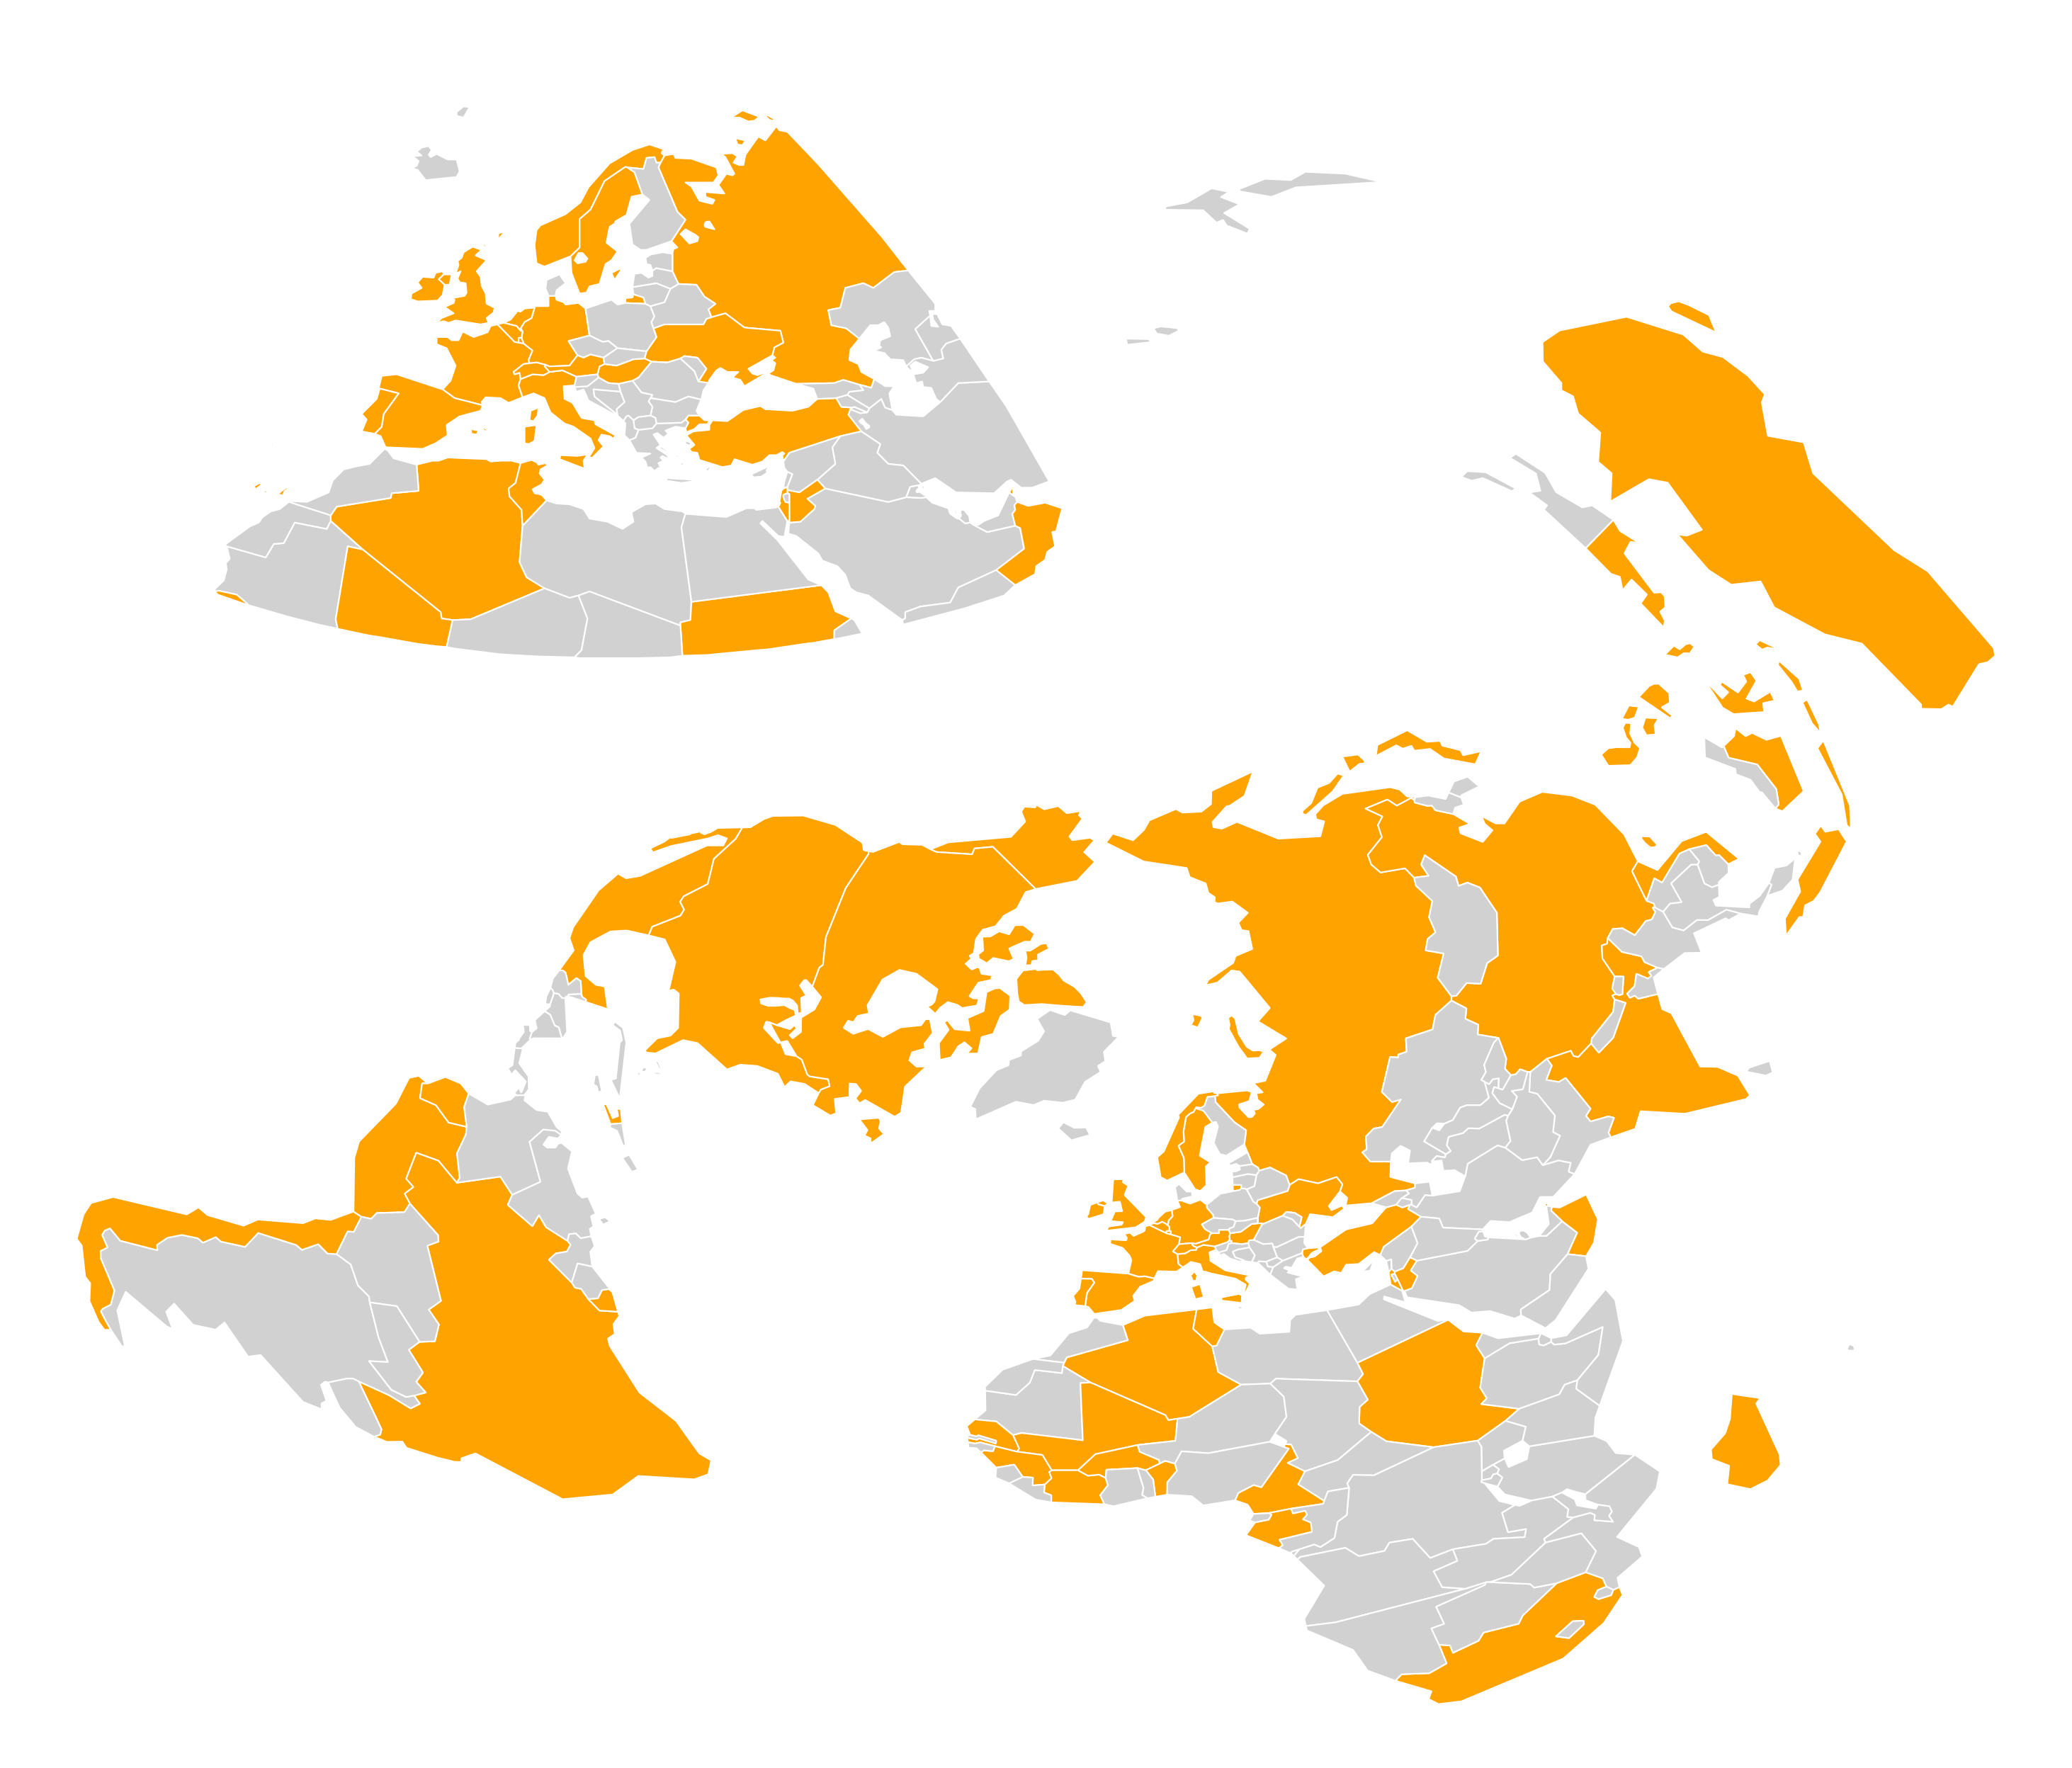
\includegraphics{Figures/CybergeoNetworks/authoring.png}
	%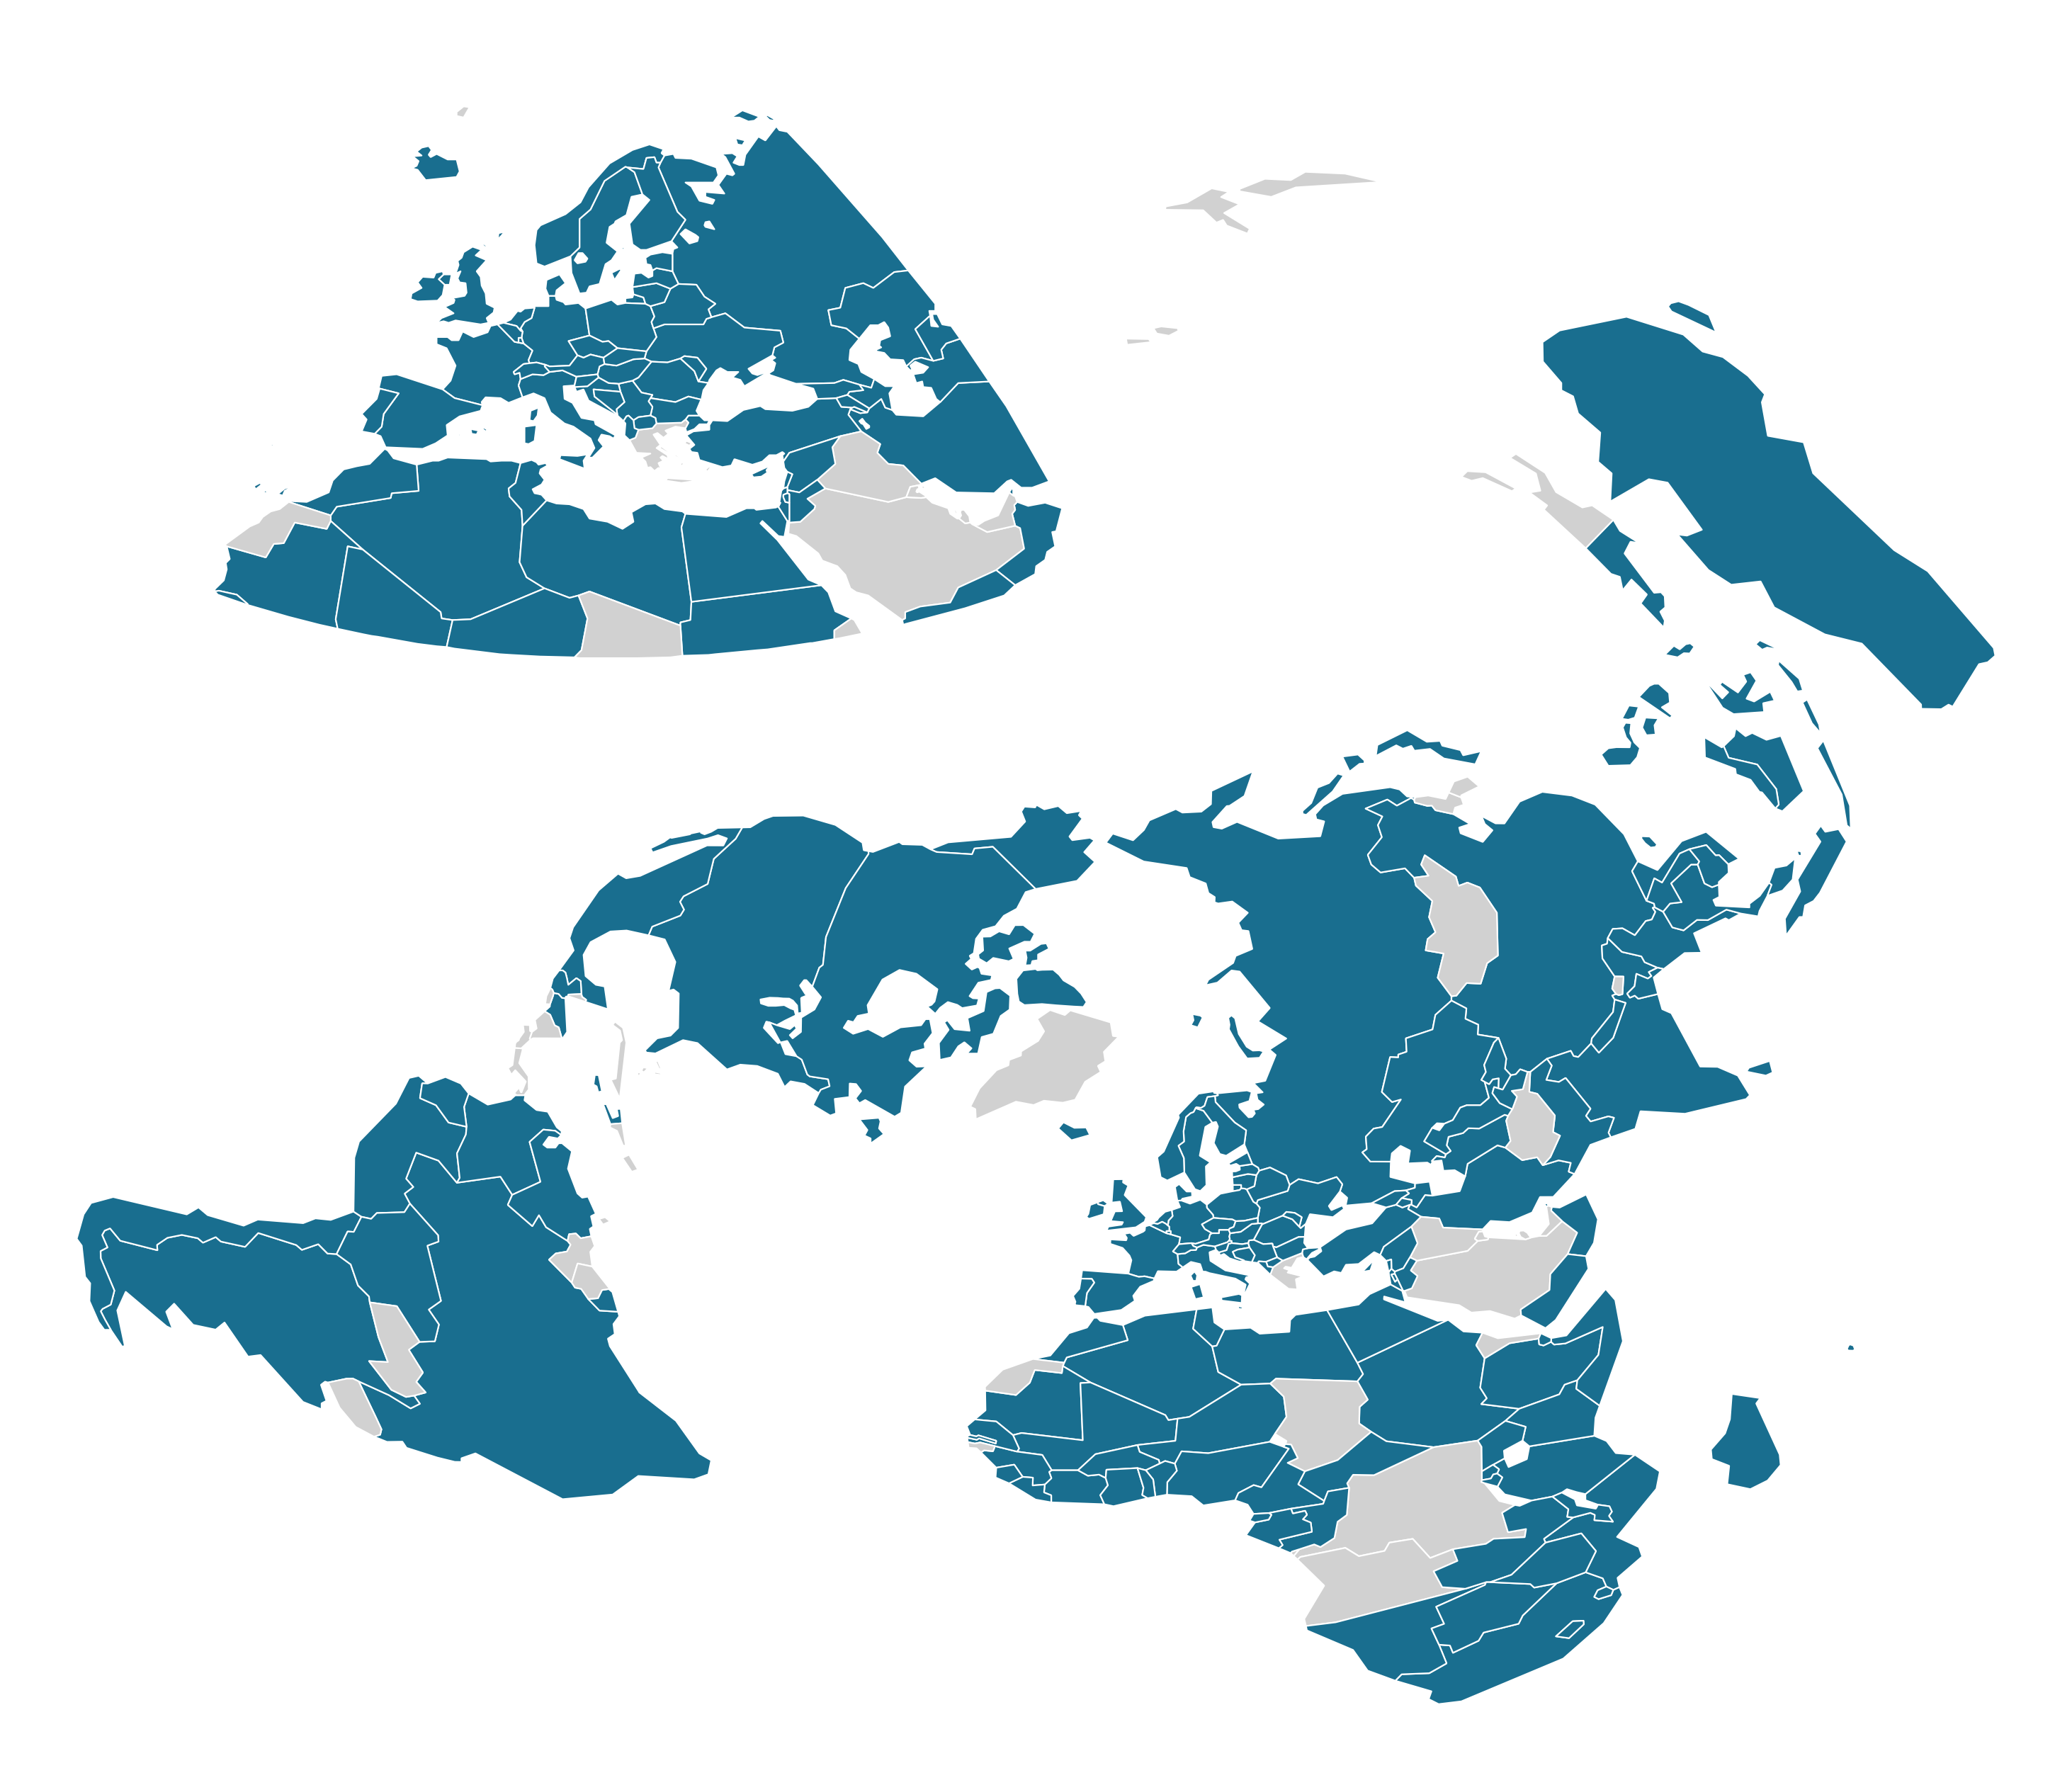
\includegraphics{Figures/CybergeoNetworks/studied.png}
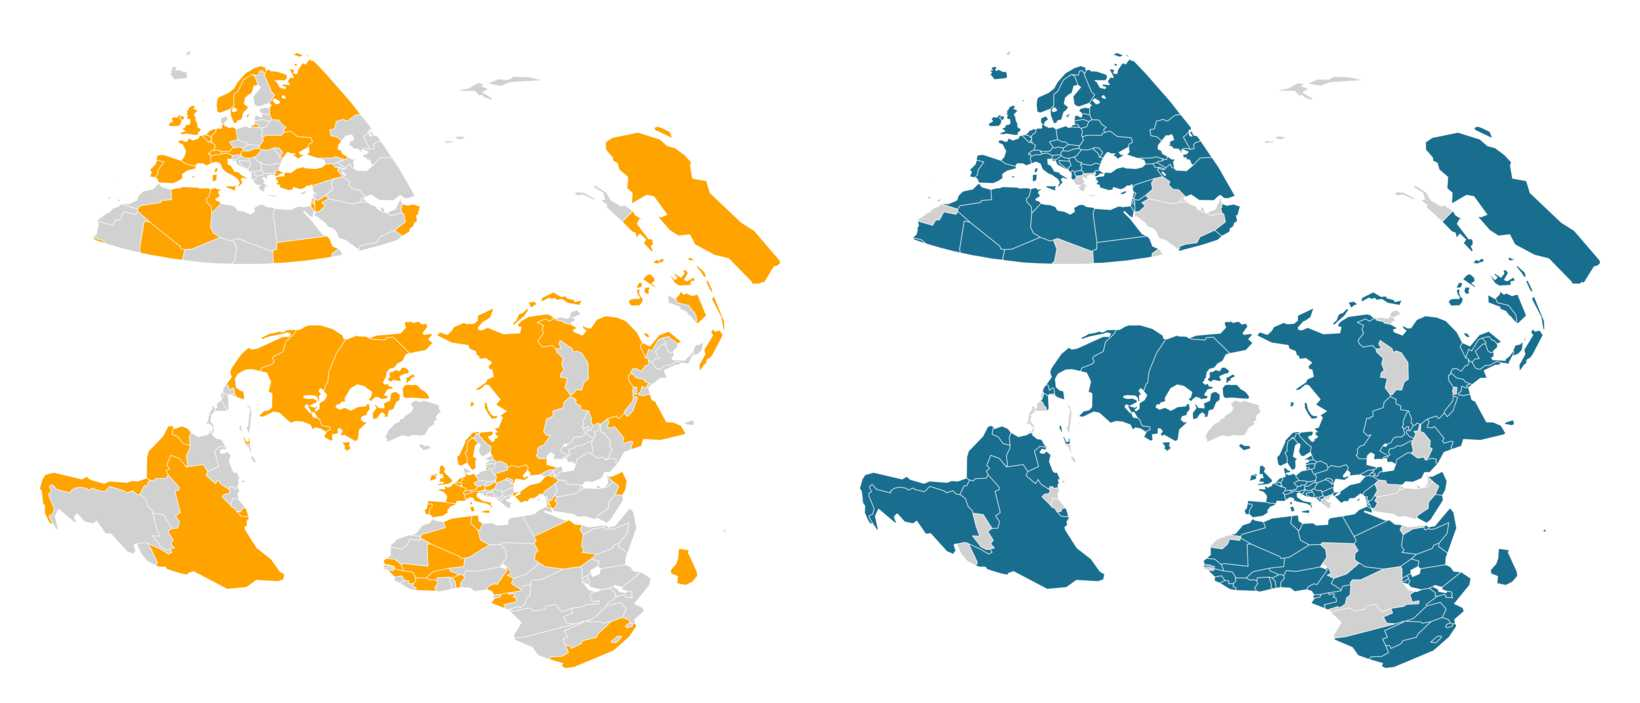
\includegraphics[width=\linewidth]{Figures/Final/C-cybergeonetworks-authoring-studied.jpg}
\appcaption{\textbf{Countries with at least one author | 1996-2015} (\textit{Left}), \textbf{Countries studied at least once | 1996-2015} (\textit{Right})\label{fig:app:cybergeonetworks:authoring}}{\textbf{Pays avec au moins un auteur, 1996-2015} (\textit{Gauche}) ; \textbf{Pays étudiés au moins une fois, 1996-2015} (\textit{Droite})\label{fig:app:cybergeonetworks:authoring}} 
\end{figure} 
%%%%%%%%%%%%%%%%%%%

%%%%%%%%%%%%%%%%%%%
\begin{figure}%[htbp] 
%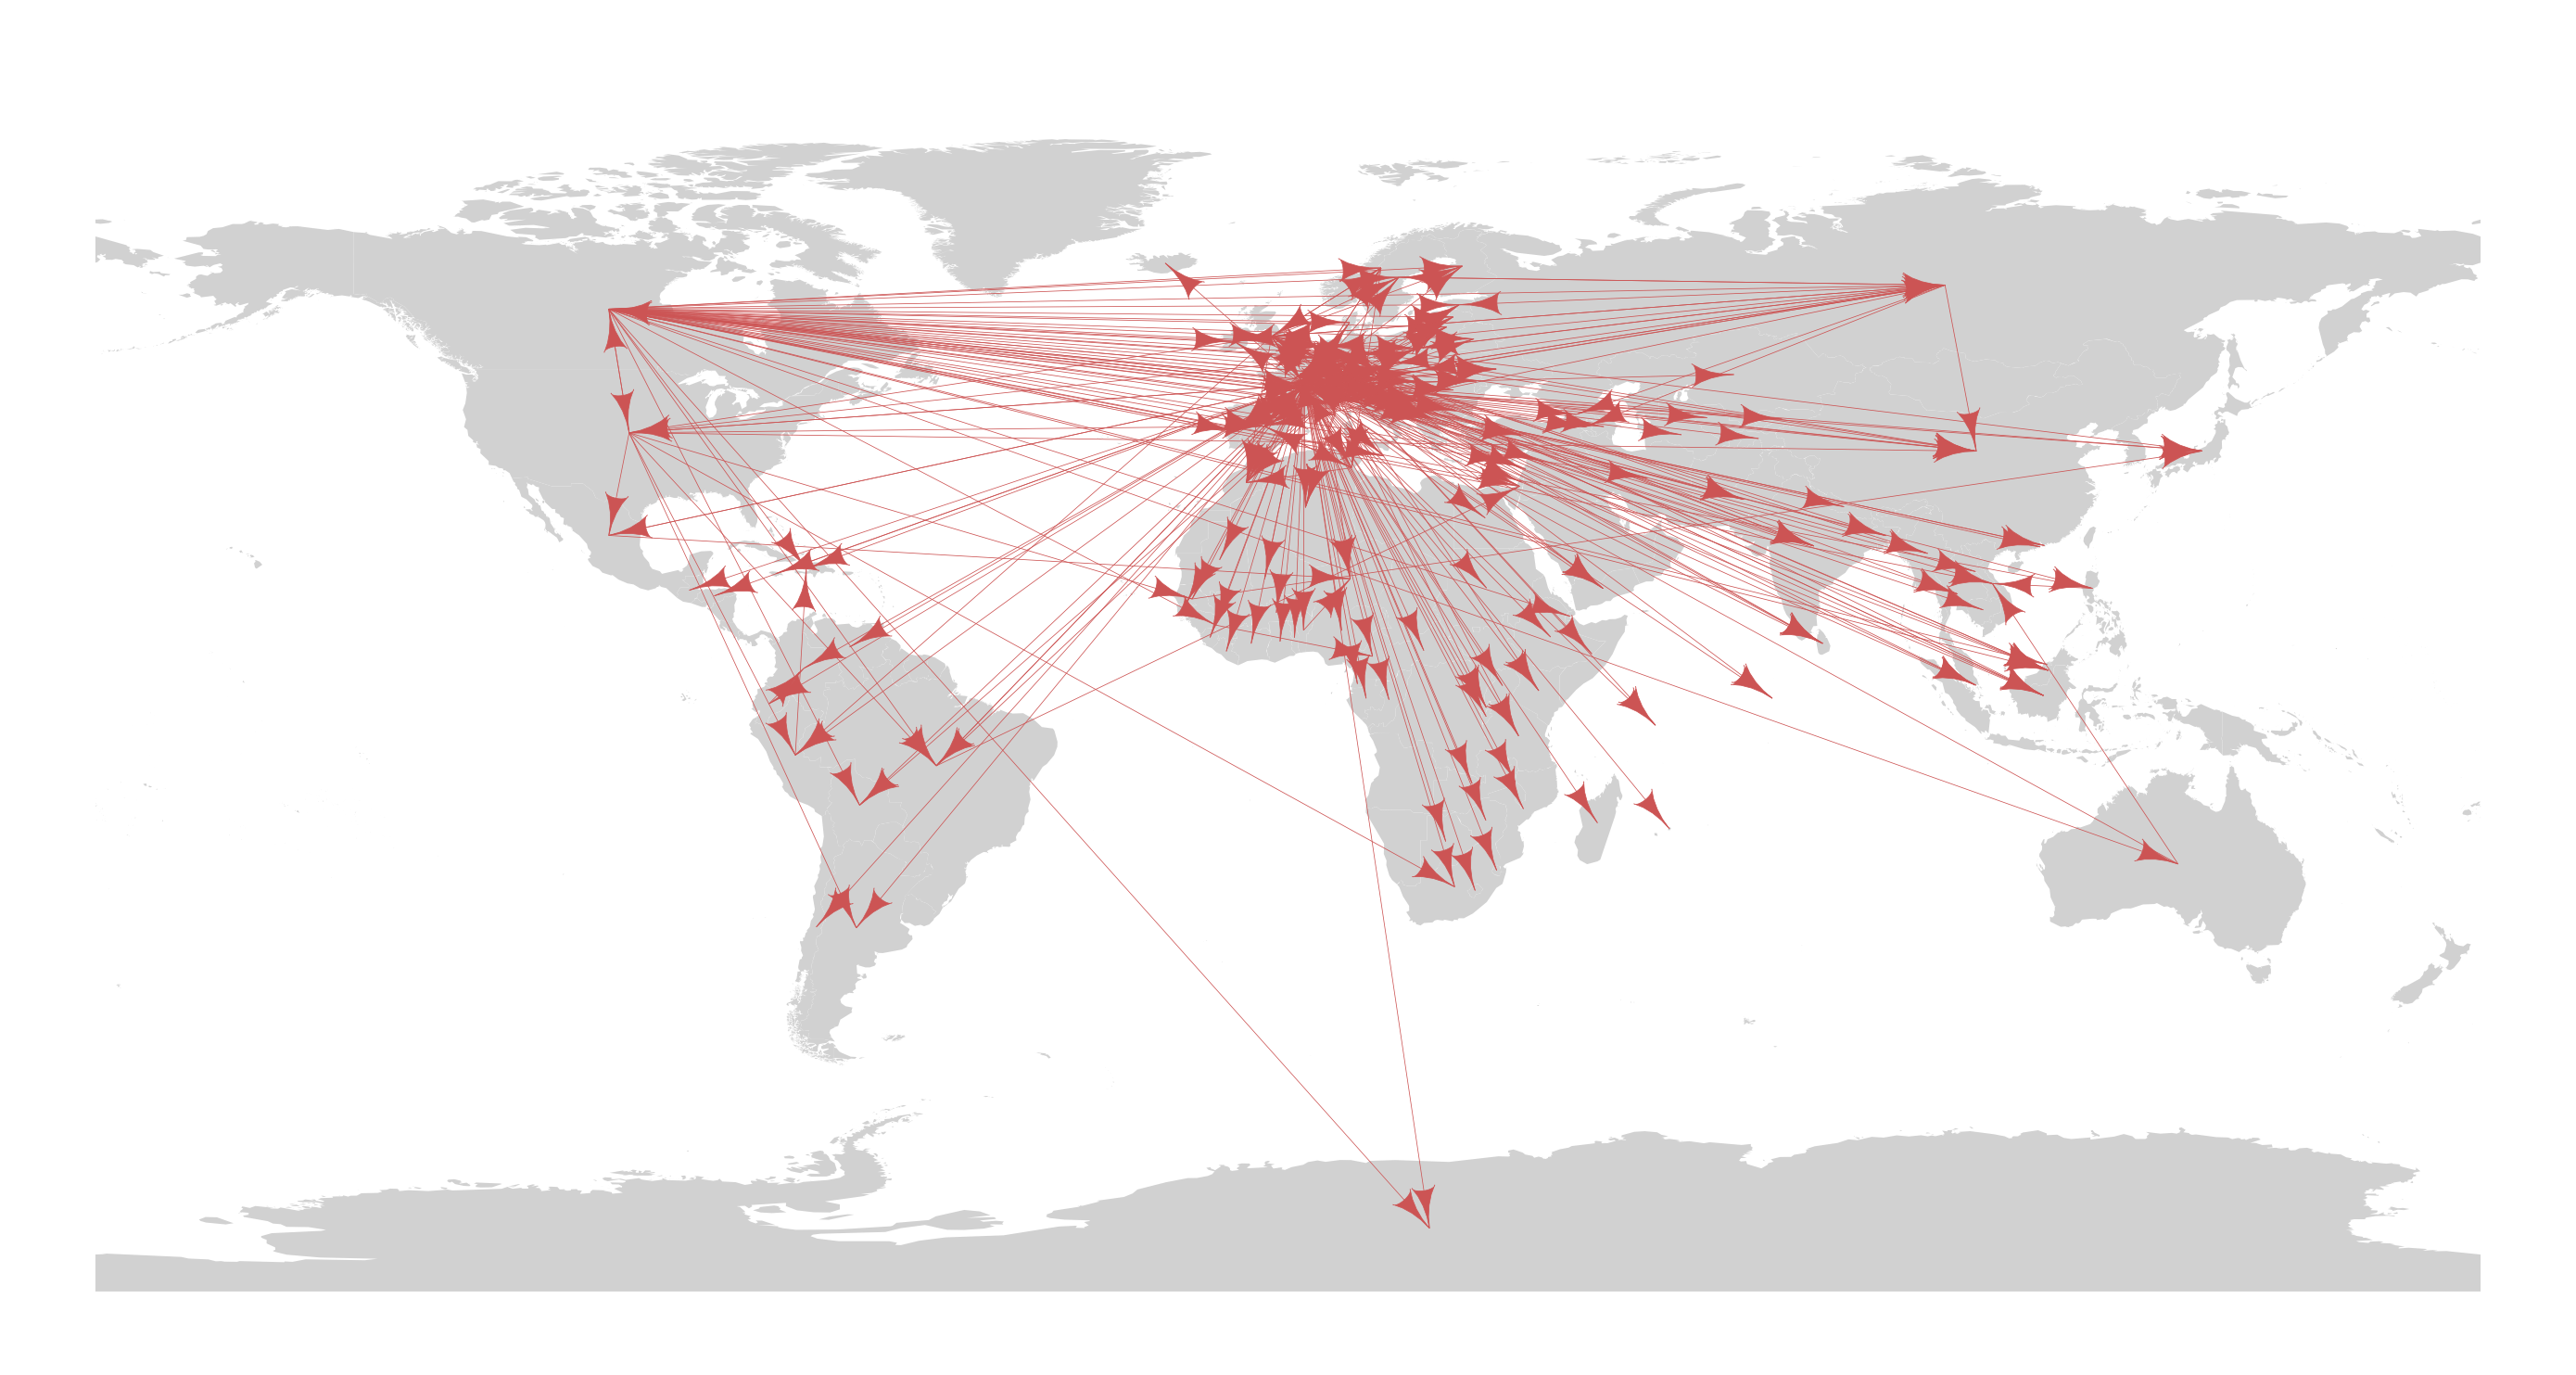
\includegraphics[width=\linewidth]{Figures/CybergeoNetworks/whoStudiesWho.png}
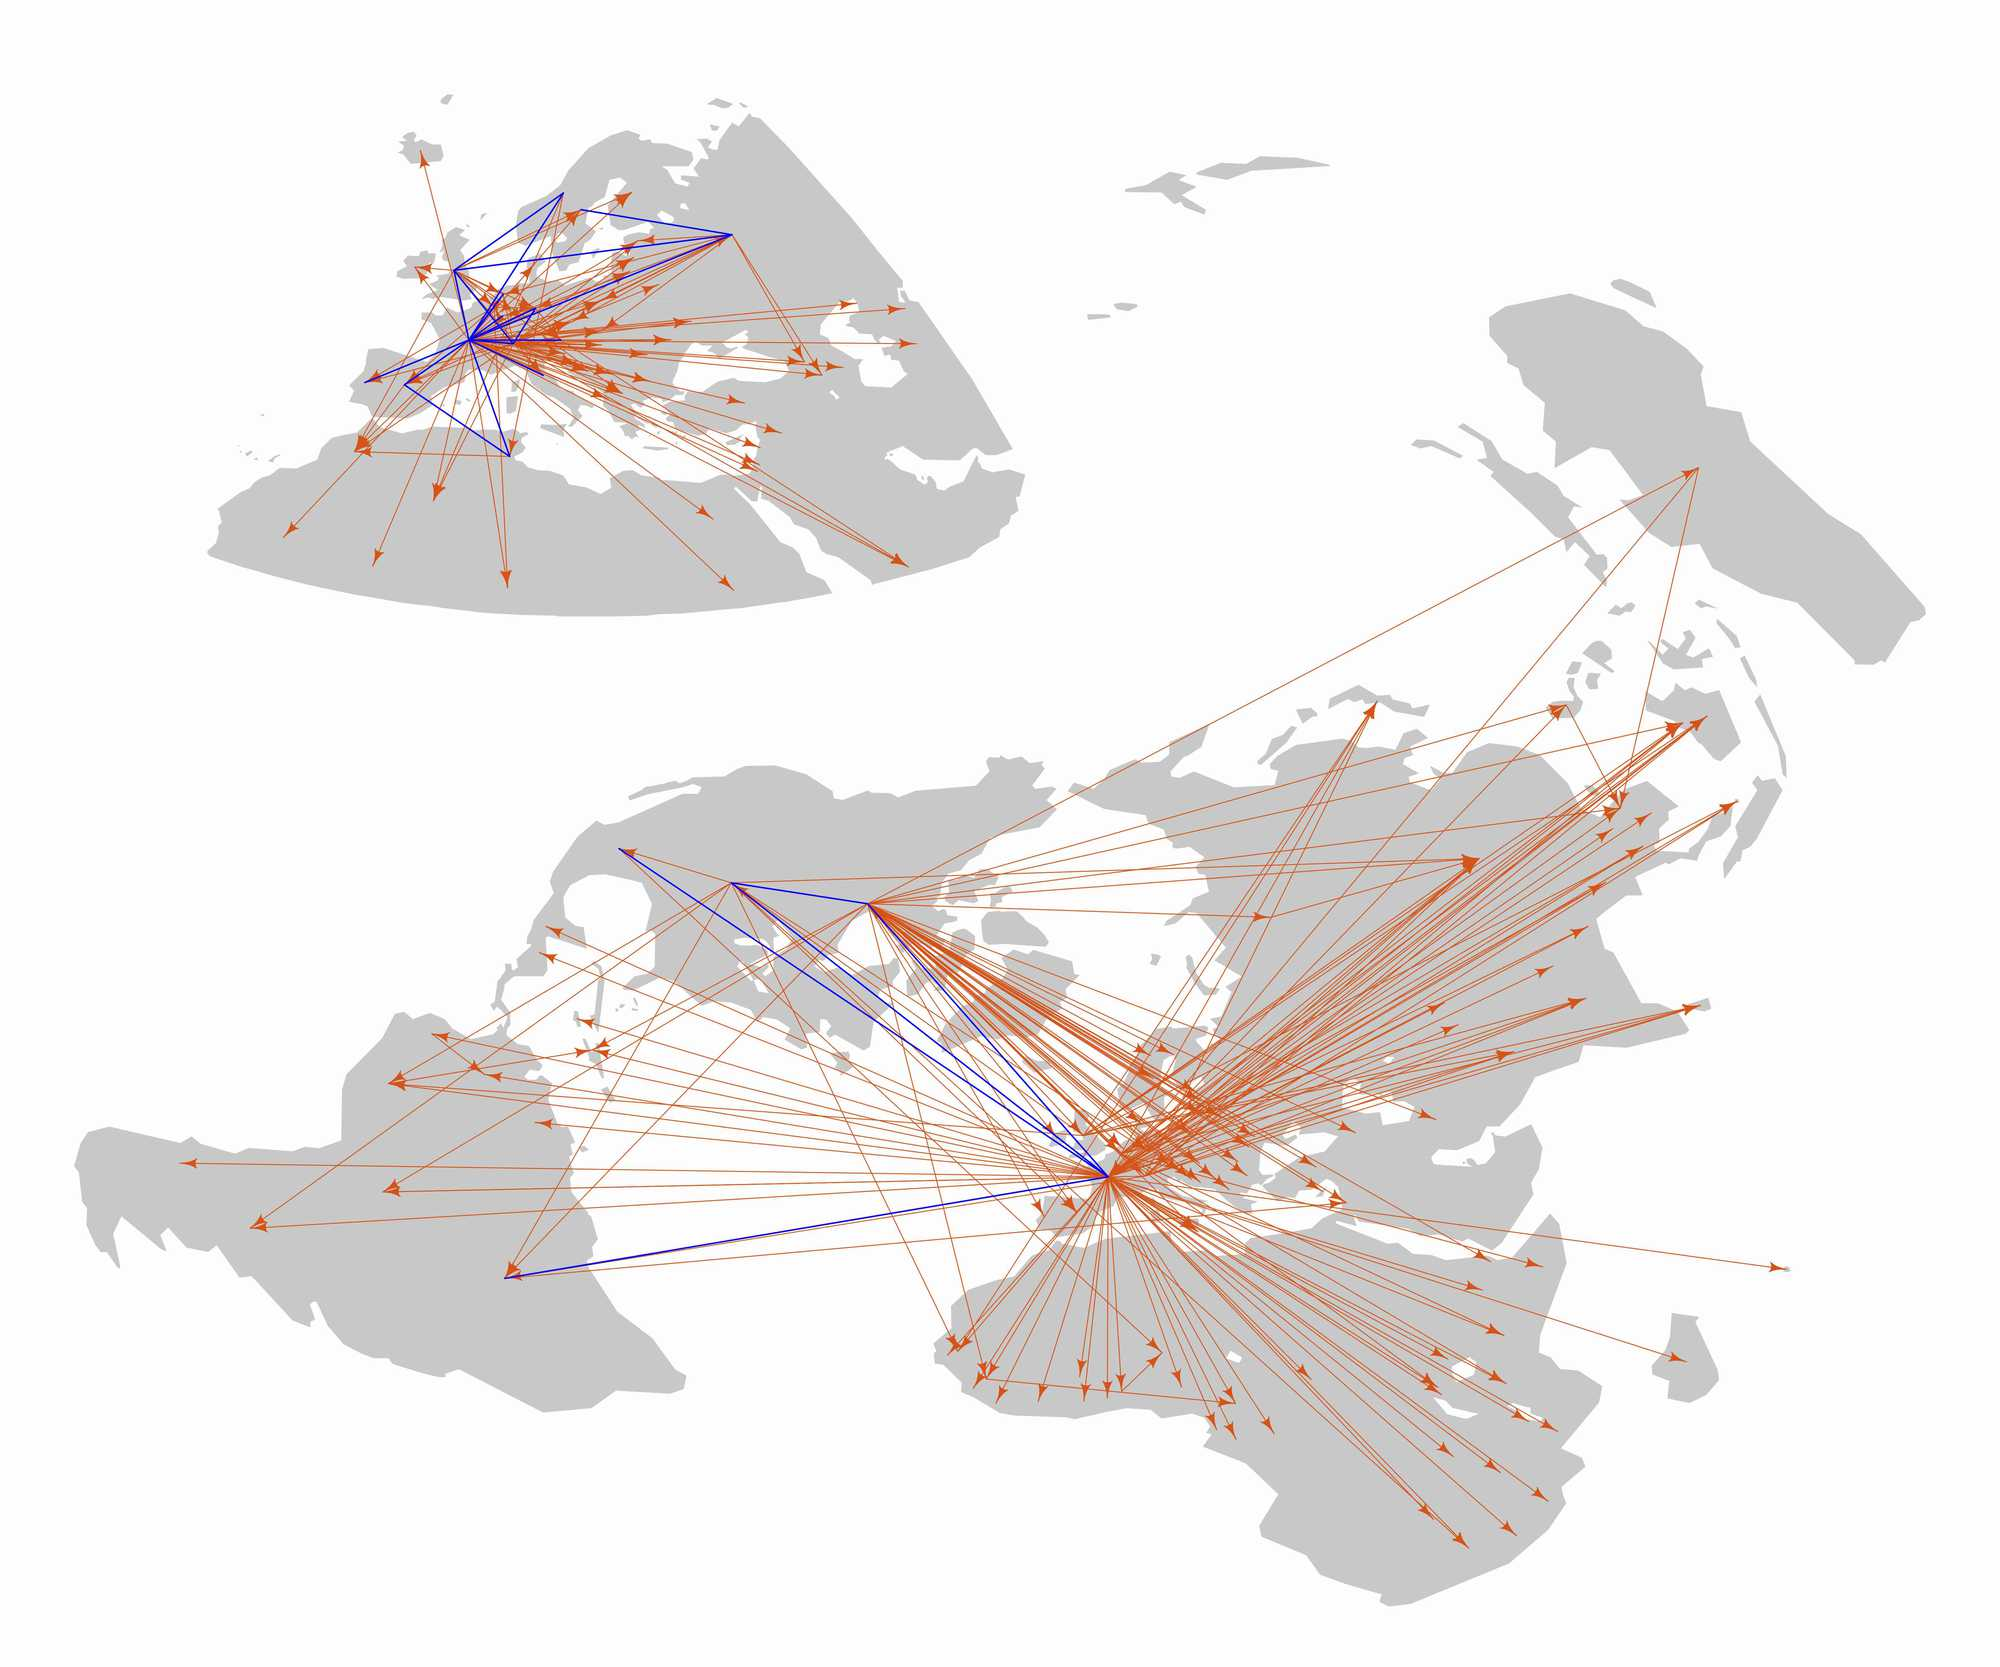
\includegraphics[width=\linewidth]{Figures/Final/C-cybergeonetworks-who.jpg}
\appcaption{\textbf{Geographical origins and destinations of papers, 1996-2015}\label{fig:app:cybergeonetworks:who}}{\textbf{Origine géographique et destination des articles, 1996-2015}\label{fig:app:cybergeonetworks:who}}
\end{figure} 
%%%%%%%%%%%%%%%%%%%

%%%%%%%%%%%%%%%%%%%
\subsection{Methods}{Méthodes}
%%%%%%%%%%%%%%%%%%%%%

\bpar{
One main aspect of our contribution is the complementary combination of different methodologies, each having its potentialities and pitfalls, but also specific questions and objects of study. We detail in this section the different methods and how they are coupled to produce new knowledge.
}{
Un aspect principal de cette contribution est la combinaison complémentaire de différentes méthodologies, chacune ayant ses potentialités et limitations, mais aussi des questions et des objets d'étude spécifiques. Nous détaillons dans cette section les différentes méthodes et comme celles-ci sont couplées pour produire une nouvelle connaissance.
}

%%%%%%%%%%%%%%%%
\subsubsection{Internal semantic network}{Réseau sémantique interne}

\bpar{
The first exploration method is based on the set of keywords declared by the articles' authors in the Cybergeo journal. We consider articles and keywords as a bipartite network. This network can be decomposed in two simple networks: a network of articles (vertices) linked by common keywords (edges); a network of keywords (vertices) linked by common articles (edges) \citep{roth_social_2010}. We consider the second one as a semantic network. 
}{

}

\bpar{
The vertices (keywords) are described by two variables: frequency and degree. The frequency is the number of articles citing the keyword. The degree is the total degree of the vertices in the network, that is, the number of edges linking a given keyword to the others (there is no distinction between in- and out- degree as the network is undirected). Both variables are distinct but correlated. The edges are described by three variables: observed weight, expected weight and modal weight. For two given keywords the observed weight is the number of articles citing both keywords. The expected weight is the probability that the edge exists considering only the vertices' degree:
\begin{equation}
\nonumber
  P_{i \rightarrow j} = \frac{w_i w_j}{w(w - w_i)} ~~~~~~~  P_{j \rightarrow i} = \frac{w_i w_j}{w(w - w_j)}
\end{equation}

\begin{equation}
\nonumber
P_{i \leftrightarrow j} = P_{i \rightarrow j} \cup P_{j \rightarrow i}
\end{equation}

\begin{equation}
\nonumber
w_{i \leftrightarrow j}^e = \frac{w}{2} P_{i \leftrightarrow j}
\end{equation}
The probability of a link between $i$ and $j$ ($P_{i \rightarrow j}$) is defined as the cross-product of the marginal sums ($w_i$ and $w_j$) divided by the total weight ($w$). This can be seen as a quasi-modularity measure or a quasi chi-squared distance. The only difference is the null diagonal that creates asymmetric probabilities. The expected weight ($w_{i \leftrightarrow j}^e$ is the product of the probability and the mid-sum of weights. Eventually the \textit{modal weight} is computed as a ratio between the observed weight and the squared-root expected weight of the edge (such as a Pearson residual in a chi-square analysis of a contingency table). This modal weight can be used as a preferential attachment measure. 
}{

}

\bpar{
Based on this preferential attachment measure two kinds of visualisations are proposed: semantic fields and communities. The semantic field shows a any given keyword at the centre of the plot and all its neighbours at a distance inversely proportional to the modal weight. The communities are computed with the Louvain algorithm \citep{blondel_fast_2008}. This community detection method is chosen among others because it is based on the modularity such as the modal weight above defined.
}{

}

%%%%%%%%%%%%%%%%
\subsubsection{External semantic network}{Réseau sémantique externe}

\bpar{
The second methodological development focus on the combination of citation network exploration with network semantic analysis. The method applied for this development is described in details by~\cite{raimbault2017exploration}. Citation Networks have been widely used in studies of science, for example as a predictive tool for the success of a paper~\citep{2013arXiv1310.8220N}, or to unveil emerging research fronts~\citep{shibata2008detecting}. Indeed, the bibliography of a paper contains a sort of scientific positioning, as a heritage to which it aims to contribute and which fields it is based on. The other way, reverse citations, i.e. contributions citing a given paper, up to a given level, shows how the knowledge produced was understood, interpreted and used, and in particular by which field (on this point the interesting example of \cite{jacobs2016death}, heavily cited today by most of quantitative studies of the city by physicists, shows how unexpected the type of the audience can be).
}{

}

% note : ca serait amusant de faire cette étude ciblée plus détaillée sur les domaines qui utilisent Jacobs, et de quelle façon (l'intuition étant que tous les physiciens citent Jacobs sans l'avoir lu...)

%\todo{Denise: "il manque une information sur: où les articles citant ont été collectés et comment est definie la « citation neighborhood of a corpus » mentionnée au début du 2e paragraphe. Même s’il y a des choses « inavouables » il faut en donner une toute petite idée parce que le lecteur se pose inévitablement la question. On peut rester un peu vague, parler d’un « collected corpus » ?"}[paragraphe qui suit]

\bpar{
We define the citation neighborhood of our corpus as all the articles citing articles published in \textit{Cybergeo}, all the articles citing the ones cited by \textit{Cybergeo}, and all the articles citing these ones. (having thus a network at depth 2). The citation data is collected using automatic data collection similarly to \cite{raimbault2017exploration}.
}{

}

\bpar{
Having constructed this citation neighborhood, we introduce a method to analyze its content through text mining. More precisely, we focus on the \emph{relevant} keywords of abstracts, in a precise sense, which was introduced by~\cite{chavalarias2013phylomemetic} to study the evolution of scientific fields, and later refined and scaled to big data on a Patent database by~\cite{bergeaud2017classifying}. Using co-occurrences of $n$-grams (keywords with multiple components, obtained after a first text cleaning and filtering), the deviation from an uniform distribution across texts using a chi-squared test gives a measure of keyword relevance, on which a fixed number is filtered. The weighted co-occurrence network between relevant keywords captures their second order relationship and we assume that its topology contains information on the structure of disciplines that are present in the citation network. A sensitivity analysis of community structure to network filtering parameters (minimal edge weight, minimal and maximal document occurrence for nodes) yield a robust network with optimal community structure, what allows to associate to each paper a list of keywords and corresponding disciplines. These are complementary to the declared keywords and the full text themes presented in the next subsection, as they reveal how authors position in the semantic landscape associated to the citation neighborhood, or what are their ``cultural backgrounds''.
}{

}


%%%%%%%%%%%%%%%%
\subsubsection{Topics allocation using full text documents}{Attribution de thématiques avec les textes complets}

\bpar{
The third and  last exploration method details the allocation of topics in full text documents, and is thus complementary to the previous ones that used declared keywords and relevant keywords within abstracts of the citation neighborhood. Topic classification of texts documents is an intense field of research, that have developed several algorithms. In this field, a topic is considered as a set of words frequently used together in the same document, and a text document as a mixture of topics. Following a long standing development in natural language processing from the weighting scheme of words called Term frequency-inverse document frequency (tfidf) introduced by \cite{salton_introduction_1986} to first generative probabilistic model of \cite{hofmann1999probabilistic}, \cite{blei2003latent} have lastly proposed an evolution with the Latent Dirichlet Allocation model (LDA). The LDA method consider texts in a destructured way, i.e. words proximity or words presence in a same sentence are irrelevant. Articles become thus bags of words. To alleviate the disadvantage of destructuring the text, different methods can be used. The probabilistic tagging method proposed by \cite{schmid_probabilistic_1994} and used in this article aims at categorizing each word by its function in the sentence, allowing us to filter only nouns, articles and verbs. The tagging includes also the transformation from plural forms into singular, and from conjugated verb form into infinitive. Each word is then associated with a frequency in a document, which can be weighted using the tfidf weights. We use in this article one of the many forms of \(tfidf\) given by
\[ tfidf_{t,d,D} = log(1+f _{t,d} ) \cdot log\left(\frac{N}{ f_{t,D}}\right) \]
where \(f_{t,d}\)  is the frequency of the term \(t\)  in the document \(d\), \(N\) is the total number of documents in the corpus and \(f_{t,D}\) is the number of documents \(D\) containing the term \(t\). This way, after having destructured text documents, filtered only nouns, articles and verbs, and finally weighted each word, we produce the matrix of weights per document and word in terms of topics, using the LDA model. LDA is a Bayesian hierarchical model (fig. \ref{fig:lda}). We give details of its structure in the following. This model considers three levels: corpus, document and word. Each level is defined by a set of probabilistic distributions and their parameters. Then, at the corpus level, the model has parameters \(\alpha\) and \(\beta\). \(\alpha\) is a vector of positive reals (once per topic). \(\beta\) is a matrix describing the probability of each word included in the dictionary (columns) for each topic (rows). Afterwards, at the document level, the generative process begins to draw the number of words from a Poisson distribution with parameter \(\epsilon\) and a vector \(\theta\) from a Dirichlet distribution with parameter \(\alpha\). Finally, at the word level, the topic \(z\) of the word is drawn from a multinomial distribution with parameter \(\theta\) and a word is drawn from a multinomial distribution with parameter the vector probability line of the topic \(z\) from the parameter matrix \(\beta\). All these parameters are estimated here using a Markov chain Monte Carlo algorithm, called Gibbs sampler from \cite{geman_stochastic_1984}. This algorithm generates a vast amount of draws of each parameters needed by the generative model, and produces a distribution of the value of each parameter. The main product is the \(\beta\) parameter, which is the probability of a word per topic, that can be then analyzed in order to understand the topic found in the corpus. During this process, the number of topics is a fixed parameter. In order to select an optimal number,  \cite{blei2003latent} proposed a graphical method aiming to identify the number of topics with a minimal perplexity and a maximal entropy.
}{

}

%%%%%%%%%%%%%%%%
%\begin{figure}[htbp] 
%\begin{center} 
%\resizebox{0.5\textwidth}{!}{ 
%	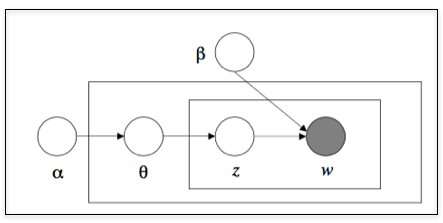
\includegraphics{figures/lda.png}
%} 
%\appcaption{Bayesian multilevel model of the Latent Dirichlet allocation (LDA) [source: \cite{blei2003latent}} 
%\label{fig:lda} 
%\end{center} 
%\end{figure} 
%%%%%%%%%%%%%%%%


%%%%%%%%%%%%%%%%
\subsubsection{Geographical aggregation of semantic profiles}{Aggregation géographique des profils sémantiques}


\bpar{
In order to produce the maps in figures \ref{fig:authoring} to \ref{fig:who} and analyses at the country level, articles have been geo-tagged in two ways. Firstly, the country of affiliation of the author(s) has been coded following the 2-letter identifiers of the International Organization for Standardization. Secondly, the articles were read one by one to extract the major geographical subjects. Articles were tagged with a country if this country or a sub-region of it constituted the focus of the study. In the case of European countries, different sets of countries were associated with the publication, depending on the perimeter of the subject (for instance: EU15, EU25, Schengen area, EuroMed, etc.). Given a semantic characterisation of articles (using keywords, citations or full-texts), it is then possible to determine two semantic profiles of countries: one using countries as authoring origins and one using countries as subject 'destination'. This semantic profile of a country X is made of the mean share of themes Y present in articles authoring from or studying country X. At one extreme, if only one article $A_1$ came from a country $X_1$, the semantic profile of $X_1$ would be exactly that of $A_1$. At the other extreme, if all articles came from $X_2$, the semantic profile of $X_2$ would be the overall distribution of themes across articles. All in all, given the three semantic characterisations of articles (using keywords, citations and full-texts) and the two geographical allocation of articles (authoring or studied), each country has a maximum of six distinct semantic profiles. We use these semantic profiles to cluster countries. The clustering method applied is an ascending hierarchical clustering algorithm using the Ward criterion of distance maximisation. When analysing authoring clusters, we consider groups of countries from which a certain geography is made and written. This option is interesting in a reflexive aspect but practically more hazardous because of the high concentration of emission and the consequently low number of emitting countries. Therefore, in the results section, we base our clustering on studied countries. When analysing clusters of studied countries, we consider how certain groups of territories are studied, what words authors use to talk about them and in which research areas the papers about them are used. 
}{

}



%%%%%%%%%%%%%%%%
\subsubsection{Open data + interactivity = reproducibility \& transparency}{Open Data + interactivité = reproductibilité \& transparence}


\bpar{
Last but not least, our methodological contribution is also closely linked to issues of reflexivity, transparency and reproducibility in the process of knowledge production. It is now a well sustained idea that all these aspects are closely linked and that their strong coupling participates to a virtuous circle enhancing and accelerating knowledge production, as seen in the various approaches of Open Science~\citep{fecher2014open}. For example, open peer review is progressively emerging as an alternative way to the rigid and slow classical canons of scientific communication: \cite{10.12688/f1000research.11369.1} proceeds to a systematic review on the notion to give an unified definition and understand its potential benefits and pitfalls. In the domain of computational science, tools are numerous to ensure reproducibility and transparency but require a strict discipline of use and are not easily accessible~\citep{wilson2017good}. Open Science suggest transparency of the knowledge production process itself, but also of the knowledge communication patterns: on this point we claim that interactive exploration of quantitative epistemological patterns are necessary. We build therefore an interactive application to allow the exploration of heterogeneous scientific corpuses.
}{

}


\bpar{
The web application is available online at \url{http://shiny.parisgeo.cnrs.fr/CybergeoNetworks/}. Source code and data, both for analyses and the web application, are available on the open \texttt{git} repository of the project at \url{https://github.com/AnonymousAuthor3/cybergeo20}.
}{

}


%\todo[JR]{faire pointer le domaine cybergeonetworks.org vers l'IP du labo (le server shiny est déjà configuré pour l'accepter comme point d'entrée), comme ça on sera un peu plus anonyme que avec l'adresse parisgeo.}[(JR) en fait un whois donne Denise Pumain sur le domaine cybergeonetworks.org, donc malheureusement pas anonyme non plus]





%%%%%%%%%%%%%%%%%%%%%
\subsection{Results}{Résultats}
%%%%%%%%%%%%%%%%%%%%%


%%%%%%%%%%%%%%%%%%%%%
\subsubsection{Internal semantic network}{Réseau sémantique interne}
\paragraph{Communities and semantic fields}{Communautés et champs sémantiques}

\bpar{
The community detection algorithm finds a modularity optimum with 10 clusters: mobility and transportation; imagery and GIS; climate and environment; history and epistemology; sustainability, risk, planning; Economic geography; Territory and population; urban dynamics; statistics and modelling; emotional geography. Some clusters concentrate a large number of keywords and articles, such as "imagery and GIS" or "statistics and modelling". This result was expected because of the original aim and scope of the journal. Beside the main clusters and a set of medium-sized clusters, two small and totally unexpected clusters emerged: "emotional geography" and "climate and environment". The CybergeoNetworks application proposes a set of visualisation parameters to draw the communities (see Figure~\ref{fig:app:cybergeonetworks:commintern}) such as setting the size of vertices and edges according to different variables (degree, number of articles, modal weight).
}{

}

%%%%%%%%%%%%%%%%%%%%%
\begin{figure}%[htbp] 

\appcaption{\label{fig:app:cybergeonetworks:commintern}}{\label{fig:app:cybergeonetworks:commintern}}
\end{figure}
%%%%%%%%%%%%%%%%%%%%%

\bpar{
The above explained modal weight metrics can be used to draw semantic fields. The CybergeoNetworks application proposes the full list of keywords. The user chooses one keyword from that list, the word is placed is the centre of the plot and all its neighbours are arranged at a distance inversely proportional to the preferential attachment (modal weight). The application proposes visualisation parameters such as setting the character size according to the weight of the keywords (number of articles or degree in the network) (see Figure~\ref{fig:app:cybergeonetworks:commintern}). Some proximities are expected ("urban" is closely linked to "city"), some are expected knowing the original scope of the journal in the field of theoretical and quantitative geography ("model" or "spatial statistics" are linked to "city"). Some proximities are totally unexpected: for "city" the preferential attachment of keywords like "movie", "web", "virtual".
}{

}


%%%%%%%%%%%%%%%%%%%%%
\begin{figure}%[htbp] 
%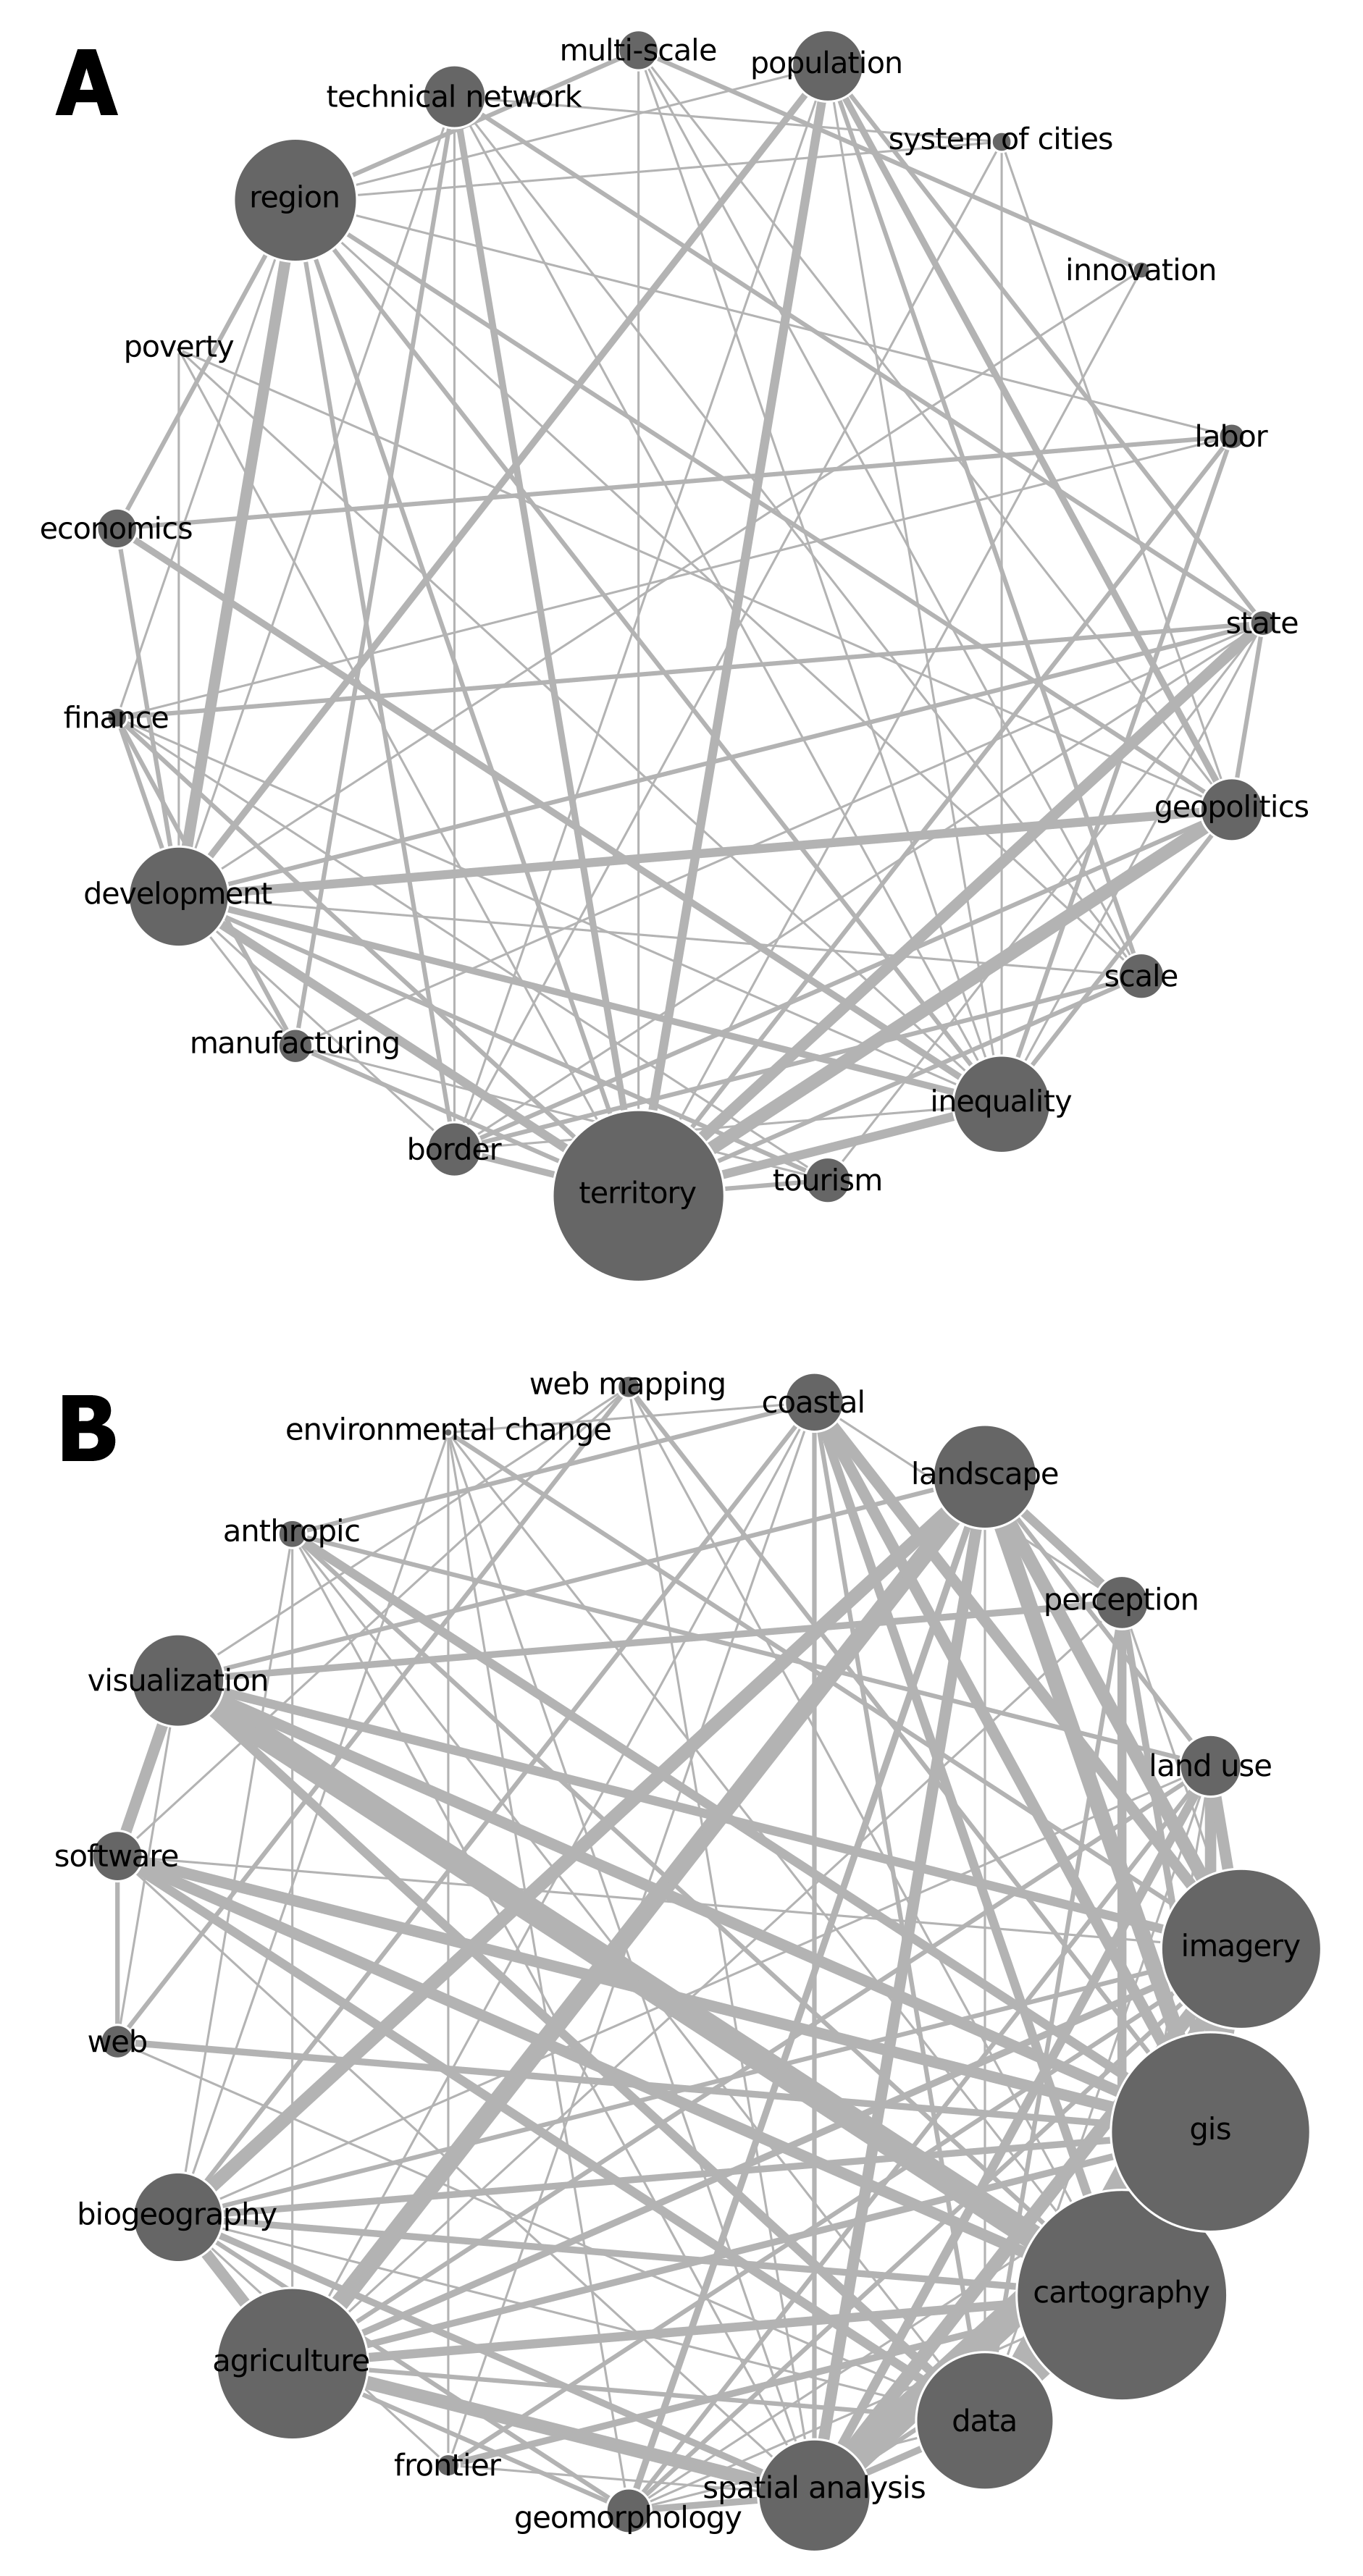
\includegraphics[width=0.45\linewidth]{Figures/CybergeoNetworks/CommunitiesVertical.png}
%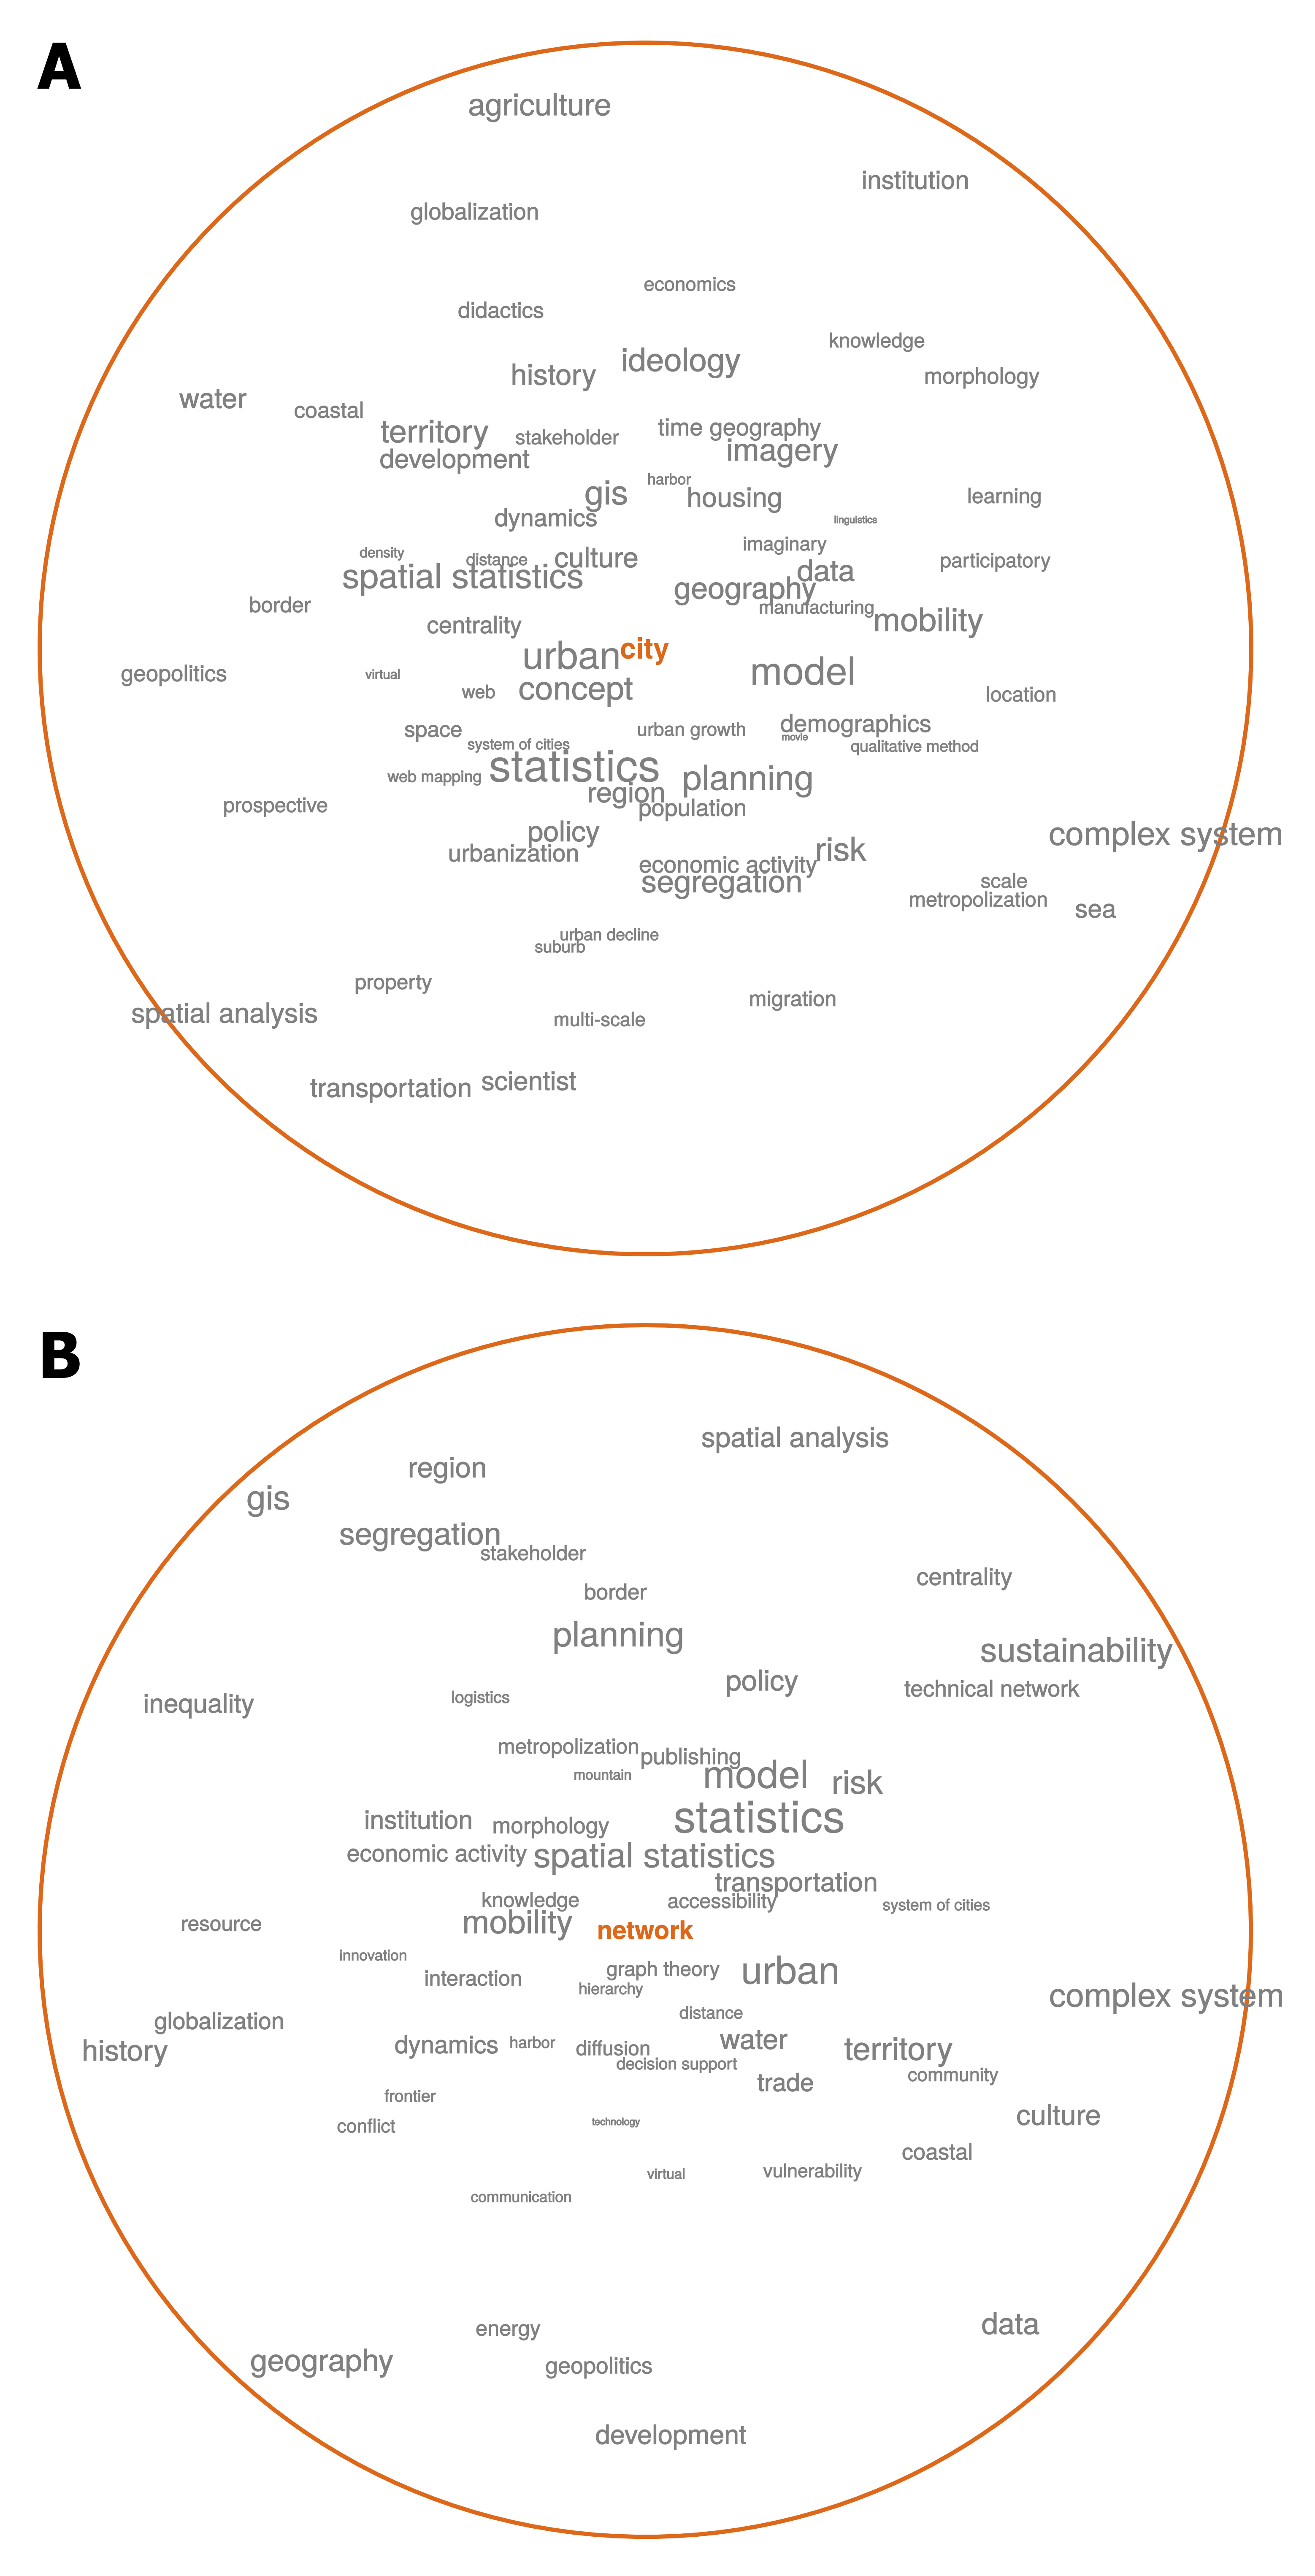
\includegraphics[width=0.45\linewidth]{Figures/CybergeoNetworks/Semantic.png}
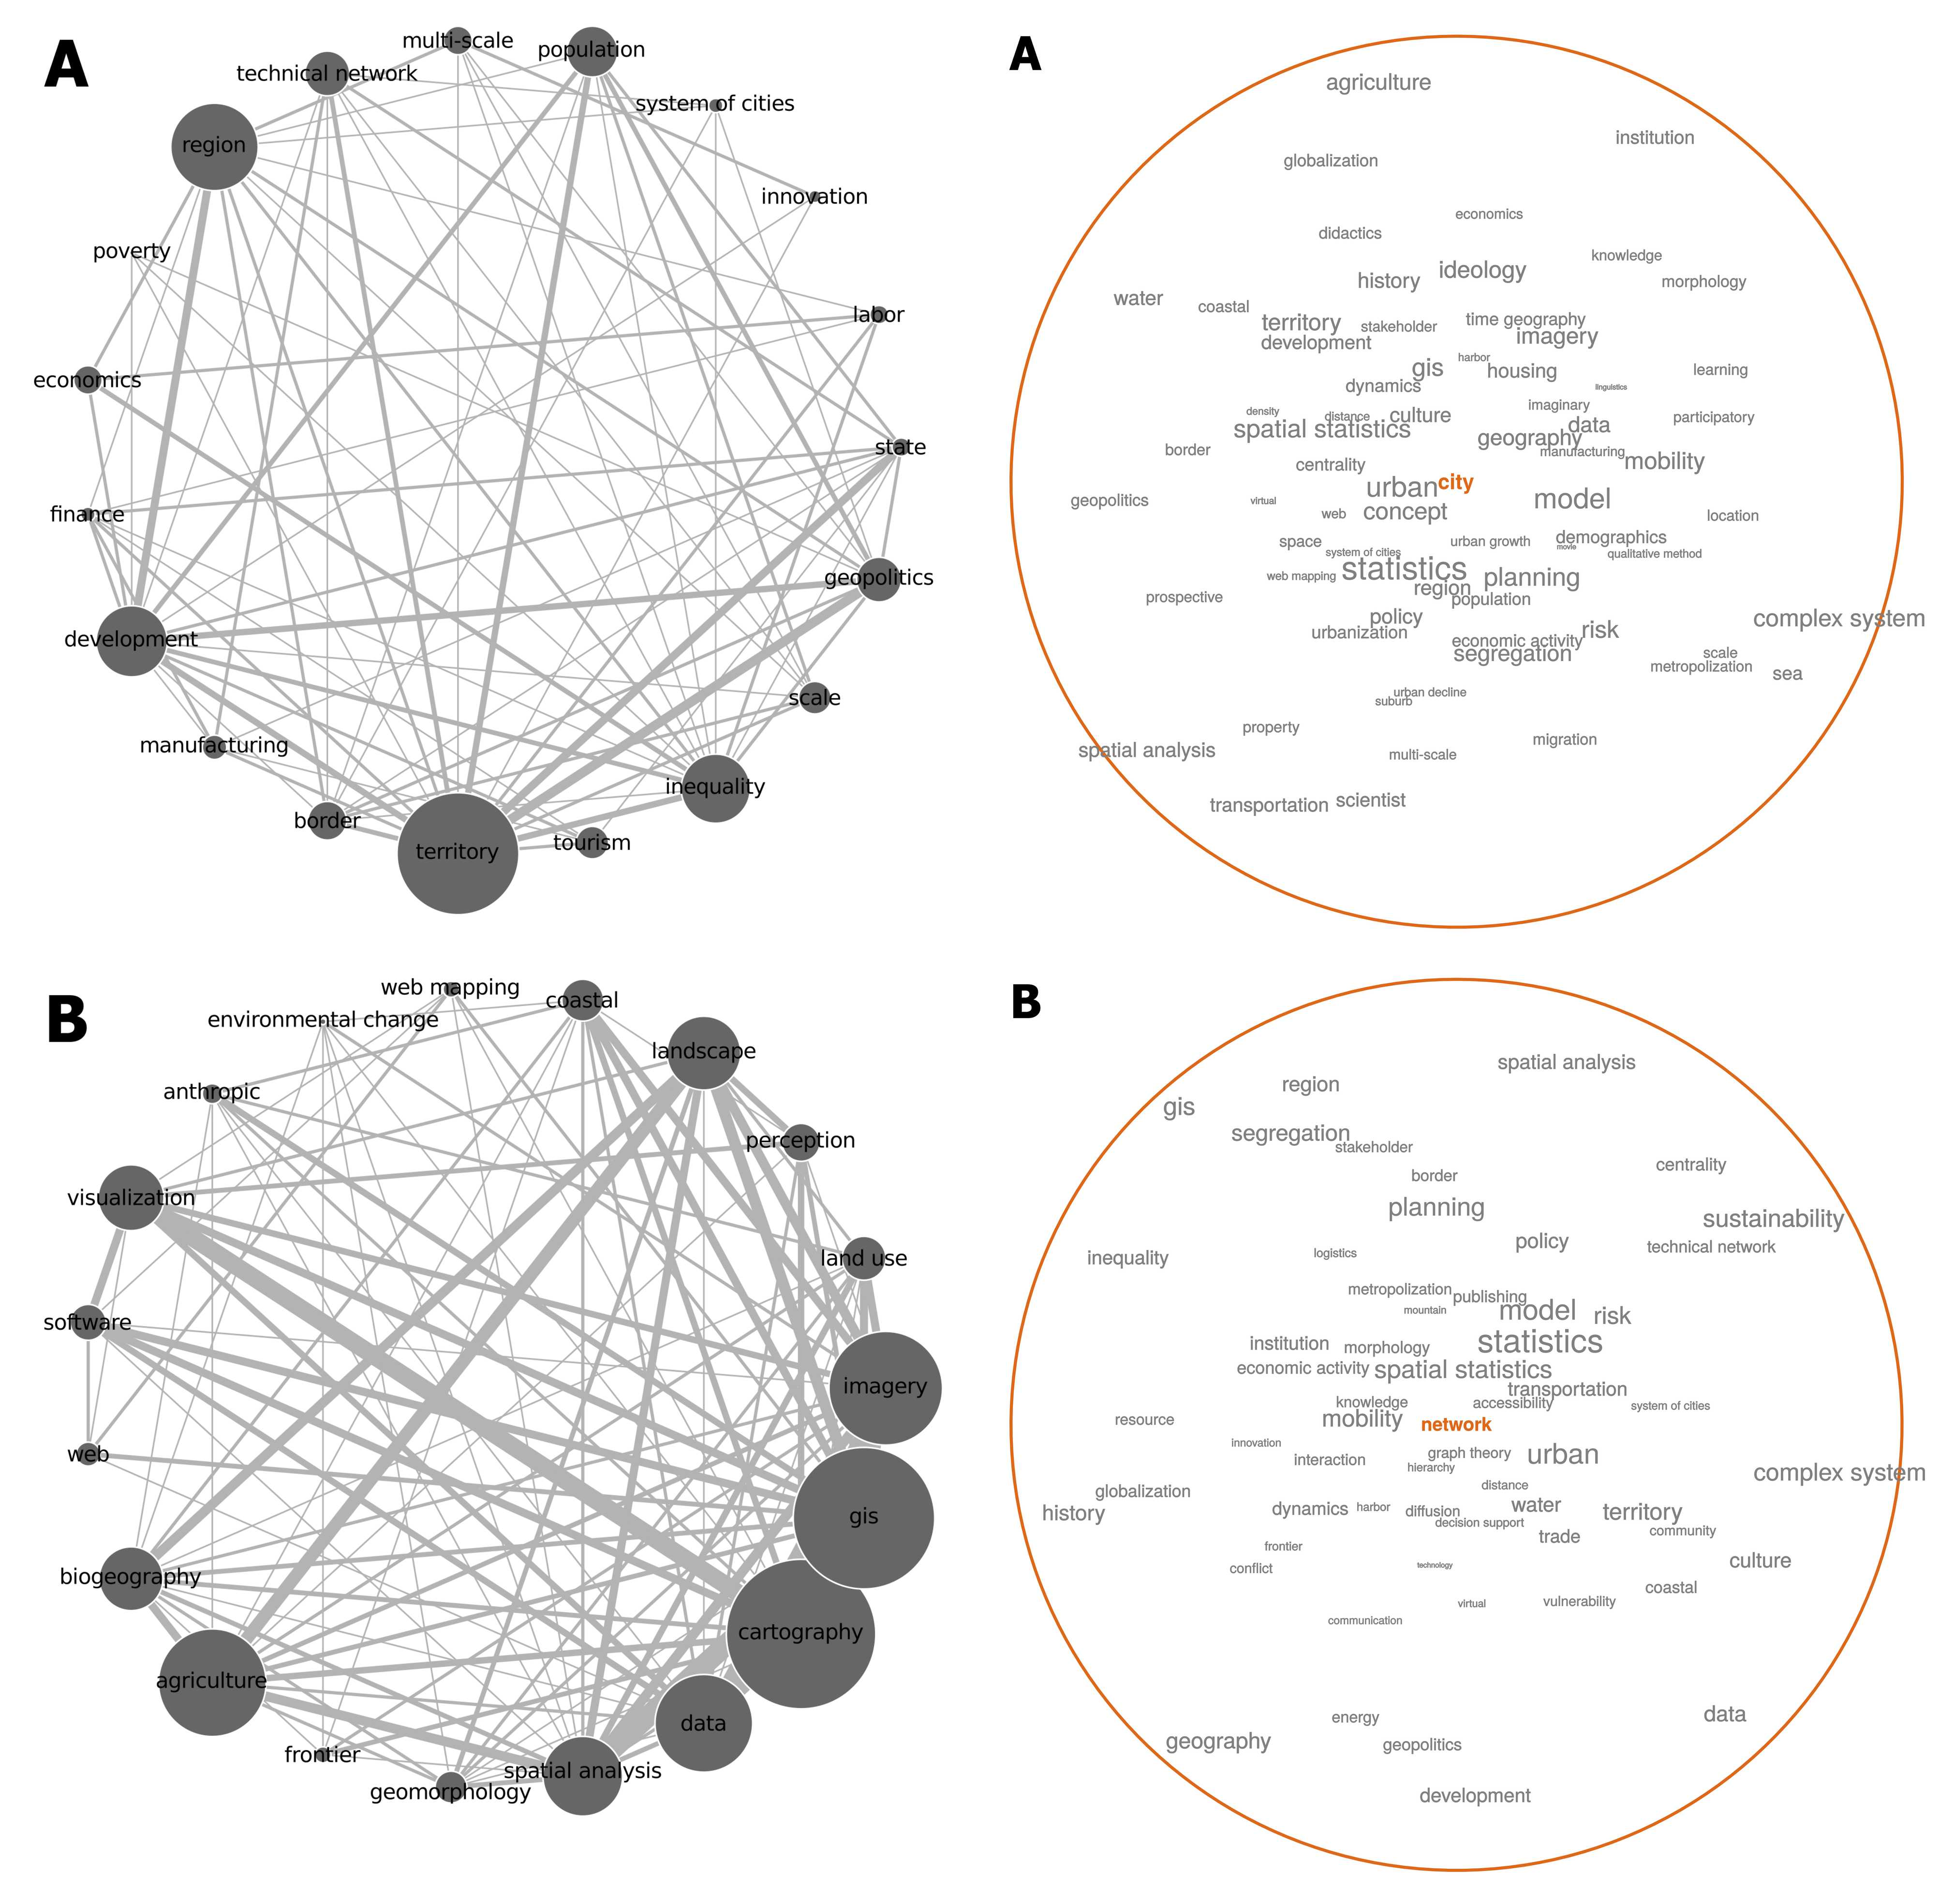
\includegraphics[width=\linewidth]{Figures/Final/C-cybergeonetworks-commintern.jpg}
\appcaption{\textbf{Community structure of the internal semantic network.} (A-Territory; B-Imagery \& GIS).\textbf{Semantic fields.} (A-City; B-Network)\label{fig:app:cybergeonetworks:commintern}}{\textbf{Structure de communauté du réseau sémantique interne : } A-Territory, B-Imagery \& GIS (\textit{Gauche}) ; \textbf{Champs sémantiques : } A-City, B-Network (\textit{Droite})\label{fig:app:cybergeonetworks:commintern}}
\end{figure}
%%%%%%%%%%%%%%%%%%%%%

%%%%%%%%%%%%%%%%%%%%%
\paragraph{Spatialised communities}{Communautés spatialisées}

\bpar{
Using the keywords distributions to draw the semantic profile of the 128 countries studied in a Cybergeo article, we obtain a clustering in 4 groups representing 16.5\% of the initial inertia. Its geographical distribution is shown in figure \ref{fig:cluster_hadri} and the average profile of each group is represented in figure \ref{fig:cluster_hadri}. 
}{

}


%%%%%%%%%%%%%%%%%%%%%
\begin{figure}%[htbp] 
%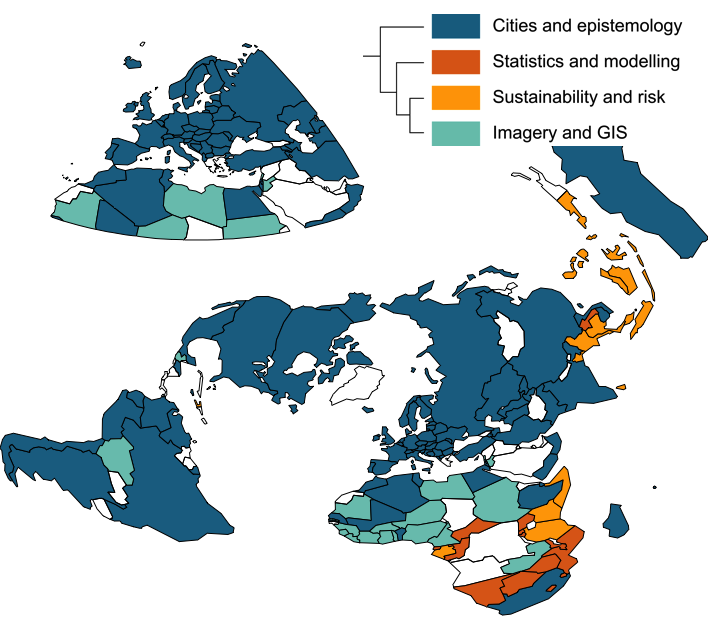
\includegraphics{Figures/CybergeoNetworks/Map_4_studied_hadri_dend.png}
%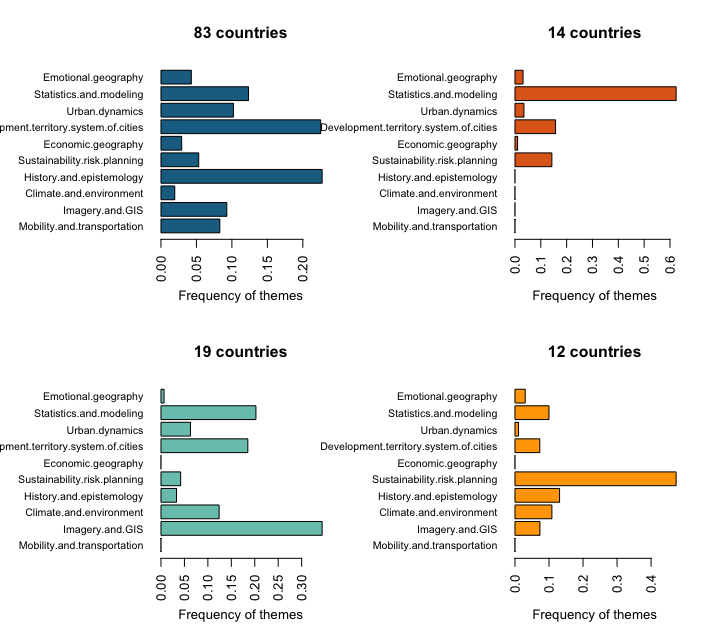
\includegraphics{Figures/CybergeoNetworks/Leg_4_studied_hadri.png}
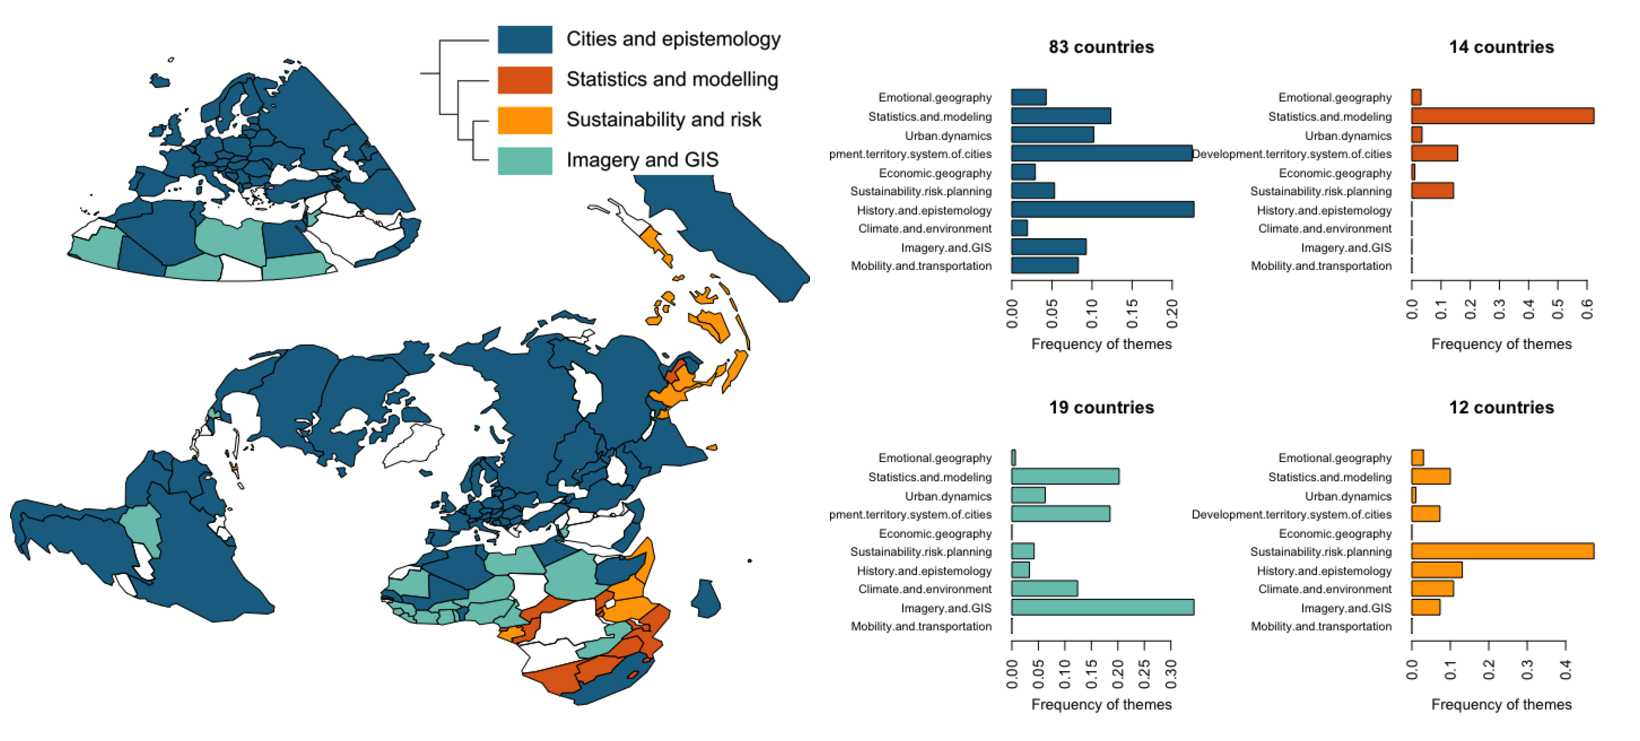
\includegraphics[width=\linewidth]{Figures/Final/C-cybergeonetworks-cluster_hadri.jpg}
\appcaption{\textbf{Geographical communities of declared interest} (\textit{Left}) ;  \textbf{Corresponding semantic profile of groups} (\textit{Right}) \label{fig:app:cybergeonetworks:cluster_hadri}}{\textbf{Communautés géographiques d'intérêt déclaré} (\textit{Gauche}) ; \textbf{Profil sémantique des groupes correspondants} (\textit{Droite}). \label{fig:app:cybergeonetworks:cluster_hadri}}
\end{figure} 
%%%%%%%%%%%%%%%%%%%%%


\bpar{
Countries are differentiated firstly by whether or not the articles studying them also declare keywords related to transport and mobility, history and epistemology, urban systems and/or emotional geography. Indeed, the first group of 83 countries (in blue, Fig.~\ref{fig:app:cybergeonetworks:cluster_hadri}) is defined by these themes. The corresponding countries are the most developed and rich territories of the world, including emergent countries such as the BRICS. The keywords used to advertise the articles about them follow the fashions of geography, with mentions of emotions and mobility for instance. 
}{

}


\bpar{
The countries of the other groups over-represent the keywords related to:
\begin{itemize}
\item methods (in orange) such as statistics and modelling. The countries associated with these keywords are all located in central and southern Africa, with the exception of Lao. These countries are studied by a small number of articles which focus on methodological approaches. For example, the only article studying Rwanda \citep{querriau2004localisation} relates to an optimal location problem whereas \citet{vallee2009disparites} uses 'multilevel modelling' as a keyword for the only article about Lao.
\item sustainability and risks (in yellow). This is the case of articles about Indonesia for example, which all relate to aleas and vulnerability: to tsunamis \citep{ozer2005tsunami}, to volcanoes \citep{belizal2011quand} and to water scarcity \citep{putra2009einfluss}.
\item Finally, 19 countries are associated with keywords related to imagery and GIS (teal colour). They are located primarily in Saharan Africa. In many cases, this happens because the articles present a methodology which uses aerial and satellite images to substitute missing socioeconomic data  \citep{ackermann2003analysis, devaux2007extraction}.
\end{itemize}
}{

}


\bpar{
Thus, drawing communities of declared interest, we find an interesting dichotomy between rich countries on the one hand, which are studied extensively in the literature and for which authors use trendy keywords to singularise themselves from past and concurrent work; and developing countries on the other hand, which are associated with more technical keywords reflecting a narrower spectrum of domains and specific data challenges.
}{

}


%%%%%%%%%%%%%%%%%%%%%
\subsubsection{External semantic network}{Réseau sémantique externe}

\bpar{
The application allows to explore the citation neighborhood of chosen articles, in terms of semantic contents (the visualisation of full networks are technically not feasible as the full corpus contains around 200,000 articles). Wordclouds give the content of the article and the content of the articles in the neighborhood, with each word being associated to the semantic communities. The user can therefore situate a work within a semantic context, and we expect that unanticipated connexions can be made with this tools, as authors may not be aware of similar works in alien disciplines.
}{
L'application permet l'exploration du voisinage de citation d'un article choisi, en termes de contenu sémantique (la visualisation des réseaux complets n'est pas faisable techniquement comme le corpus complet contient autour de 200,000 articles). Les nuages de mots donnent le contenu de l'article et le contenu des articles dans le voisinage, chaque mot étant associé aux communautés sémantiques. L'utilisateur peut ainsi situer un travail dans son contexte sémantique, et nous nous attendons à ce que des liens non anticipés puissent être faits avec ces outils, comme les auteurs ne sont pas forcément au courant de travaux similaires dans des disciplines étrangères.
}


%%%%%%%%%%%%%%%%%%%%%
\paragraph{Communities structures}{Structure des communautés}


\bpar{
As explained before, the raw semantic network is optimized for modularity and size, taking a compromise between these two opposite objectives, when edge and node filtering parameter vary. This provides 12 communities, that can correspond to existing disciplines, to methodological issues, or to very precise thematic subjects. The communities are, in order of importance in terms of proportion of total keywords : Political Science/Communication; Biogeography; Social and Economic Geography; Climate; Physical Geography; Commerce; Spatial Analysis; Microbiology; Neuroscience; GIS; Agriculture; Health. This method has the characteristic of grouping keywords by co-occurrences, revealing thus the actual structure of abstracts contents: it is both an advantage when revealing links as for the large field of Social and Economic Geography, but can also blur information by grouping more detailed communities. Very precise small communities such as Health Geography appear as they are strongly isolated from the rest of the communities. This structure is particular, and shows a dimension of knowledge that for example classical citation analysis do not reveal.
}{
Comme expliqué précédemment, la réseau sémantique brut est optimisé pour la modularité et la taille, en prenant un compromis entre ces deux objectifs opposés, tandis que les paramètres de filtrage des liens et des noeuds varient.
}

%%%%%%%%%%%%%%%%%%%%%
\paragraph{Spatialised communities}{Communautés spatialisées}


\bpar{
Using the previous networks to draw the semantic profile of the 128 countries studied in a Cybergeo article, we obtain a clustering in 5 groups representing 19.3\% of the initial inertia. Its geographical distribution is shown in figure \ref{fig:cluster_juste} and the average profile of each group is represented in figure \ref{fig:leg_cluster_juste}. 
}{

}


%%%%%%%%%%%%%%%%%%%%%
\begin{figure}%[htbp]  
\resizebox{0.5\linewidth}{!}{ 
	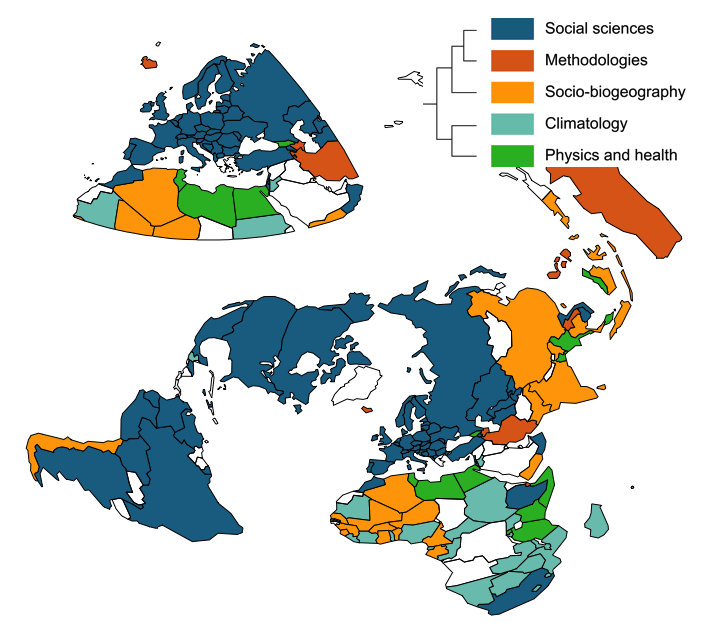
\includegraphics{Figures/CybergeoNetworks/Map_5_studied_juste_dend.png}
} 
\appcaption{\textbf{Geographical communities of bibliographical use.}\label{fig:app:cybergeonetworks:cluster_juste}}{\textbf{Communautés géographiques d'usage bibliographique.}\label{fig:app:cybergeonetworks:cluster_juste}}
\resizebox{0.5\linewidth}{!}{
	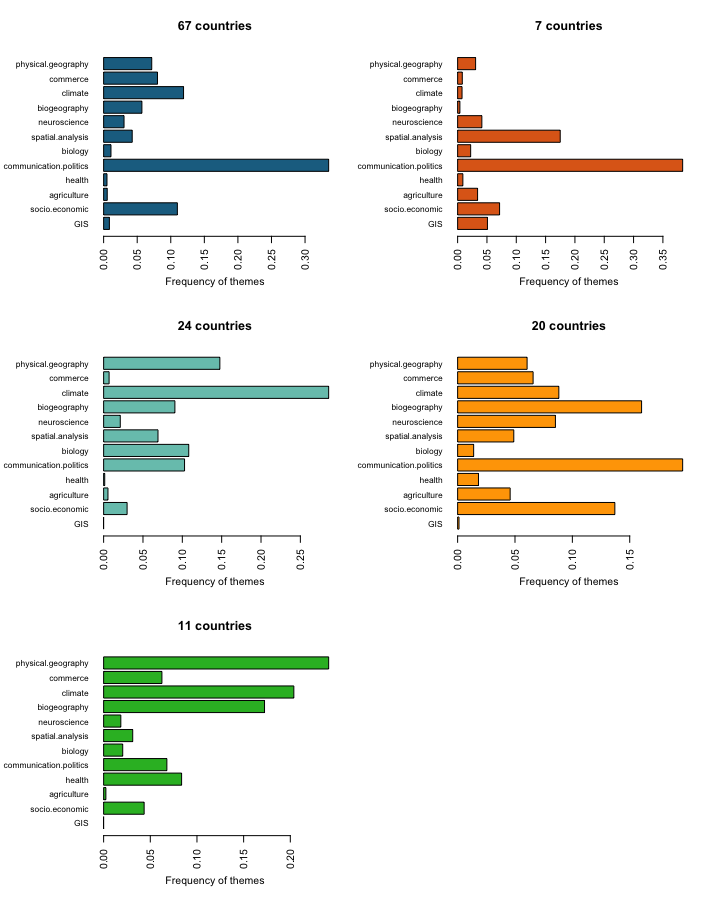
\includegraphics{Figures/CybergeoNetworks/Leg_5_studied_juste.png}
} 
\appcaption{\textbf{Corresponding semantic profile of groups.}\label{fig:app:cybergeonetworks:leg_cluster_juste}}{\textbf{Profil sémantique correspondant.}\label{fig:app:cybergeonetworks:leg_cluster_juste}} 
\end{figure} 
%%%%%%%%%%%%%%%%%%%%%


\bpar{
The largest group of countries largely overlaps with the largest cluster of keywords communities (cf. previous section). Indeed, rich and emergent countries are studied in articles used in similar ways in citation networks. There are further divides among this group. A first subgroup (in blue) of countries is studied by Cybergeo articles cited preferentially in the fields of commerce, socio-economic and politics analysis. These correspond to articles mostly in Economics and Social Sciences.
}{

}


\bpar{
The nearest subgroup of countries (in orange) comprises Australia, Azerbaijan, Iran, Lao, the Philippines and Iceland. It corresponds to countries treated by articles cited preferentially in methodological fields (spatial analysis and GIS). Indeed, the only article about Iran presents a collaborative decision support system \citep{jelokhani2012web} while the only article about Australia reviews online cartographic products \citep{escobar2000distribution}. This kind of articles then tends to stay in the citation clique of geomatics.
}{

}


\bpar{
The third subgroup refers to countries of South-East Asia, Western Africa, Yemen and Chile. The articles studying them are cited preferentially in the fields of biogeography and socioeconomic studies, although they match the average profile.
}{

}


\bpar{
In the second group of countries, we find a first subgroup of sub-Saharan countries (in teal) associated with papers cited in the climatology citation community. The second subgroup is composed of East African, North African and South-East Asian countries (in green) associated with papers cited in the fields of physical geography and health.
}{

}


\bpar{
Thus, drawing communities of bibliographical use, we find an interesting  dichotomy between rich countries on the one hand, which are associated with papers cited in broad communities, including topical and methodological fields; and poor and developing countries on the other hand, which are associated with papers cited mainly in relation to natural hazards, health and risks in the literature.
}{

}


%%%%%%%%%%%%%%%%%%%%%
\subsubsection{Topics allocation using full text documents}{Thèmes avec textes complets}

\paragraph{Evolution of the topics addressed in the corpus}{Evolution des thèmes du corpus}

\bpar{
After destructuring text documents and filtering nouns, articles and verbs, our corpus counts no less than four millions words, which leads to a dictionary of 137 224 unique words. Then, the optimal number of topics was chosen by estimating the LDA parameters with different numbers of topics: 2, 5, 10, 20, 50, 100 and 200. Similar results were obtained using a different scheme being more precise between 20 and 40. We test the robustness of results to stochasticity by iterating ten times each parameter estimation for a specific number of topics. We then consider that 20 topics is an optimal according to perplexity (fig. \ref{fig:perplexity}) and entropy (fig. \ref{fig:entropy}) indicators.\comment[JR]{il manque une étape ici (peut etre a mettre en legende des figures - je pense a rassembler en une seule) : que veulent dire ces indicateurs (facultatif), mais surtout comment sont-ils utilises pour determiner l'optimalité? (min/max/pareto ?)}
}{}

%%%%%%%%%%%%%%%%%%%%%
\begin{figure}%[htbp]
	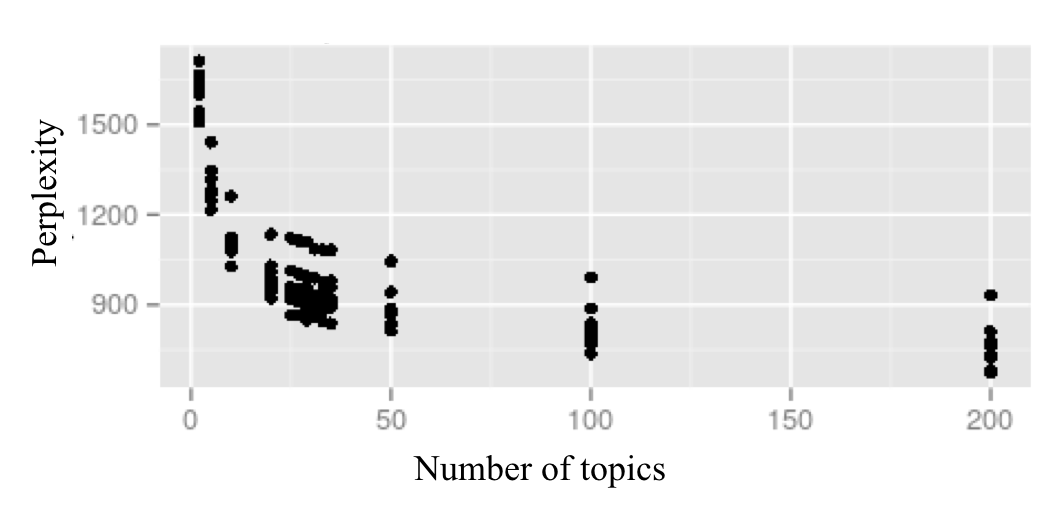
\includegraphics[width=\linewidth]{Figures/CybergeoNetworks/perplexity.png}\\
	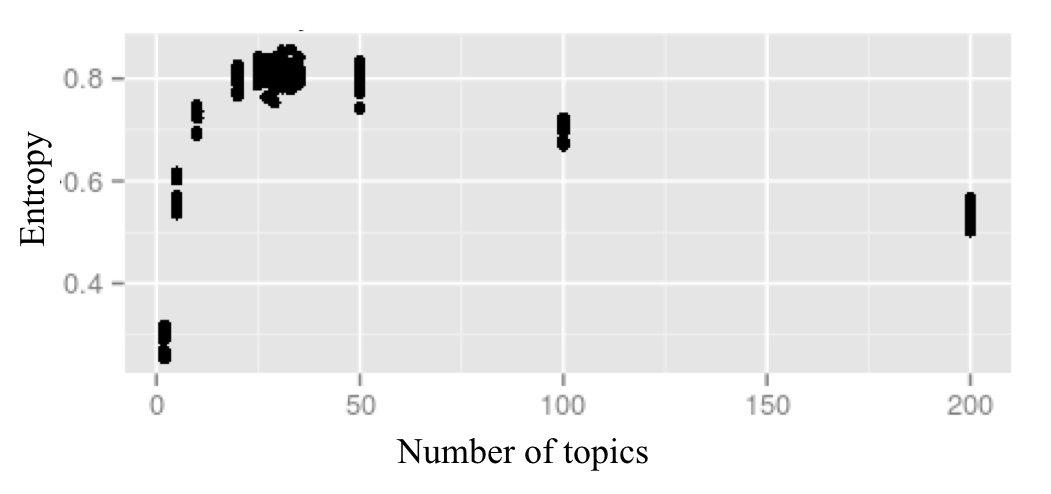
\includegraphics[width=\linewidth]{Figures/CybergeoNetworks/entropy.png}
\appcaption{\textbf{Perplexity and Entropy of the LDA model per number of topics.}\label{fig:app:cybergeonetworks:perplexity}}{\textbf{Perplexité et entropie du modèle LDA par nombre de thèmes.}\label{fig:app:cybergeonetworks:perplexity}}
\end{figure} 
%%%%%%%%%%%%%%%%%%%%%

\bpar{
The final result of the topic allocation model is the parameter matrix \(\beta\). It describes the probability \(p\) of each word of the dictionary to belong to a topic. We present below a part of this matrix describing for each topic index the translated (except for the index 7) words in decreasing order of their probability to belong to this topic (tab. \ref{tab:words-list}).
\begin{table}
\caption{List of words and its probability to belong to the topic\comment[JR]{comment doivent etre interpretees les probas ?}}
\label{tab:words-list}
\begin{tabular}{c|p{65mm}}
  Index & Words (probability) list \\
  \hline\footnotesize
  1 & district (8), city (7), housing (5), household (3) \\
  2 & move (6), mobility (5), density (4), accessibility (3), indicator (3), simulation (3), modeling (2), scenario (2) \\
  3 & image (8), soil (7), occupation (4), surface (4), vegetation (2), map (2), resolution (2), pixel (2), landscape (2), fire (2) \\
  4 & planning (7), governance (4), urban planning (2), sustainability (2), document (2), participation (2) \\
  5 & risk (9), vulnerability (5), hazard (3), flood (2), city (2), water (2), disaster (2), management (2) \\
  6 & firm (7), healthcare (3), care (2) \\
  7 & the (16), and (8), The (2), for (2), are (2) \\
  8 & index (4), agent (3), graph (2), vertex (2), mountain (2) \\
  9 & city (5) \\
  10 & water (8), exploitation (4), management (3), farmer (2), agriculture (2), parcel (2) \\
  11 & map (10), cartography (3), journal (3), http (2), image (2), atlas (2) \\
  12 & geography (8), geographer (3), author (3), document (3), science (2) \\
  13 & island (5), student (3), geography (3), education (2), identity (2), image (2), university (2) \\
  14 & city (23), agglomeration (4), metropolis (3), area (2), urbanization (2) \\
  15 & Border (3), China (2), State (2), States (2), Brazil (2), Asia (2), Nation (2) \\
  16 & vote (5), map (3), party (2) \\
  17 & village (10), Pole (3), Departement (3), Area (2), Map (2), University (2), Student (2) \\
  18 & village (5), season (2), rain (2), resort (2), valley (2), precipitation (2), speed (2) \\
  19 & landscape (9), heritage (2), image (2), tourist (2) \\
  20 & port (4), sea (3), wind (2), station (2), breeze (2), Tunis (2), temperature (2) \\
\end{tabular}
\end{table}
It is then interesting to observe how many documents addressed a topic per year, i.e. the topics evolution in the Cybergeo corpus (fig. \ref{fig:topics-evolution}). We can distinguish several evolution profile: decreasing, punctual, regular and increasing topics. Articles about cartography (11) tends to decrease. Articles about remote sensing (3) was mainly produced in 2000, just like articles about water management (10) in 2004 and 2011. Articles about agglomeration (14) are regularly produced. Topics such as district (1) and mobility (2) tends to increase.
}{

}



%%%%%%%%%%%%%%%%%%%%%
\begin{figure}%[htbp] 
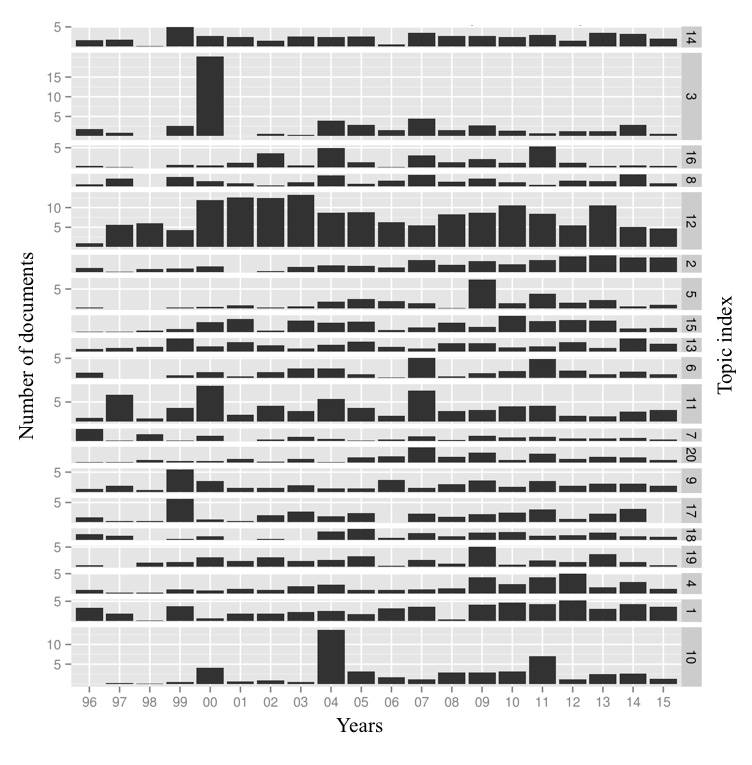
\includegraphics[width=\linewidth]{Figures/CybergeoNetworks/evolution.png} 
\appcaption{\textbf{Number of documents addressing a topic per year, between 1996 and 2015.}\label{fig:app:cybergeonetworks:topics-evolution}}{\textbf{Nombre de documents traitant d'un thème par années, entre 1996 et 2015.}\label{fig:app:cybergeonetworks:topics-evolution}} 
\end{figure} 
%%%%%%%%%%%%%%%%%%%%%


\paragraph{Spatialised full-text communities}{Communautés de texte complet spatialisées}

\bpar{
Using the full texts to draw the semantic profile of the 128 countries studied in a Cybergeo article, we obtain a clustering in 4 groups representing 13.4\% of the initial inertia. Its geographical distribution is shown in figure \ref{fig:cluster_poc} and the average profile of each group is represented in figure \ref{fig:leg_cluster_poc}. 
}{

}


%%%%%%%%%%%%%%%%%%%%%
\begin{figure}%[htbp]  
\resizebox{0.5\linewidth}{!}{ 
	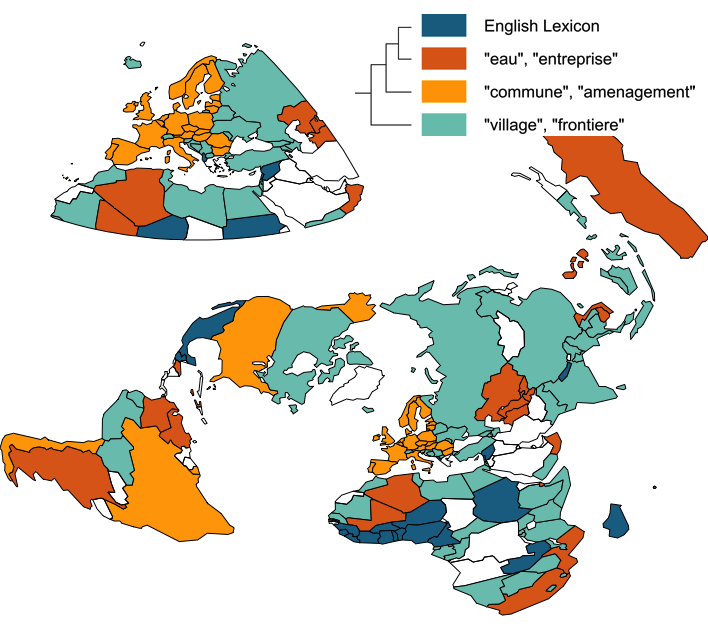
\includegraphics{Figures/CybergeoNetworks/Map_4_studied_poc_dend.png}
} 
\appcaption{\textbf{Geographical communities of writing practice.}\label{fig:app:cybergeonetworks:cluster_poc}}{\textbf{Communautés géographiques des pratiques d'écriture.}\label{fig:app:cybergeonetworks:cluster_poc}}
\resizebox{0.5\linewidth}{!}{ 
	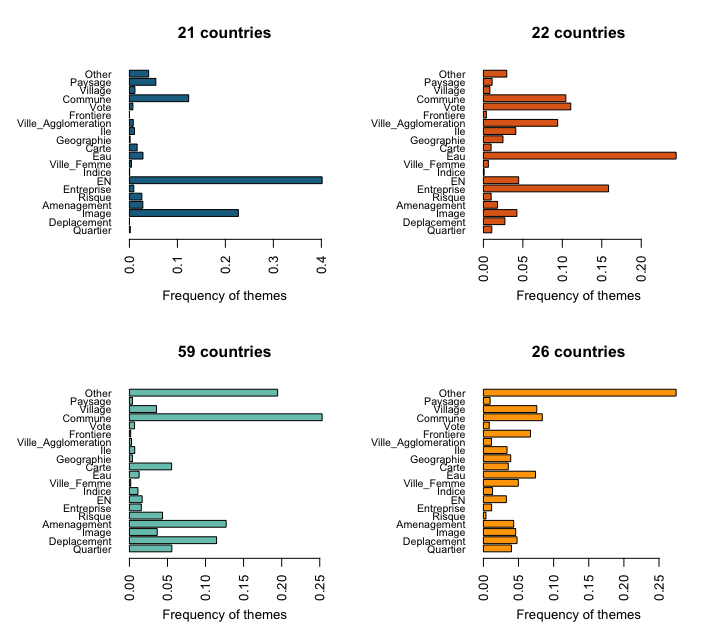
\includegraphics{Figures/CybergeoNetworks/Leg_4_studied_poc.png}
} 
\appcaption{\textbf{Corresponding semantic profile of groups.}\label{fig:app:cybergeonetworks:leg_cluster_poc}}{\textbf{Profile sémantique des groupes correspondants.}\label{fig:app:cybergeonetworks:leg_cluster_poc}}
\end{figure}
%%%%%%%%%%%%%%%%%%%%%


\bpar{
In this clustering analysis, we do not find the dichotomy of countries based on their wealth and economic development levels. The link between semantic and geographical proximity is also less obvious at the world level, although one region is strikingly revealed: the institutional boundaries of Europe. The group of countries included in the EU27 plus the USA, Brazil and Chile (in yellow) appear strongly similar in terms of vocabulary used to talk about them. In particular, themes related to issues of administrative boundaries ("\textit{communes}") and regional planning ("\textit{amenagement}") describe these countries well (for example: \citep{santamaria2009schema, lusso2009musees, le2011consommation}). Two subgroups neighbour this cluster in the clustering tree. The first one includes countries studied by papers written in English. The second subgroup includes countries from all continents and corresponds to papers written preferentially with words such as "\textit{eau}" (water) and "\textit{entreprise}" (enterprise). Finally, 59 countries are distant from these groups in that words used to write about them refer to villages and borders ("\textit{frontiere}"), in contexts as diverse as Canada, Ecuador, Malaysia or Zimbabwe. The communities of vocabulary and writing practice thus appear less straightforward and less linked to geographical proximity. The main result lays in the fact that there is a specific set of words used to write about the European Union, a sort of EU27 Novlang made of words like "Eurovision", "subsidiarity" and "Spatial Development Perspectives".
}{

}





%%%%%%%%%%%%%%%%%%%%%
\subsection{Discussion}{Discussion}
%%%%%%%%%%%%%%%%%%%%%

%%%%%%%%%%%%%%%%%%%%%
\subsubsection{Why three classifications? Evaluating the complementarity of approaches}{Evaluation de la complémentarité des approches}


\bpar{
This section backs up the previous qualitative comparison of approaches through their spatialization by quantitative measures of their complementarity. Although we have seen that the communities obtained from the three different methods are semantically and geographically distinct, we do not know precisely how they complement each other. The overlapping analysis is complicated by the fact that articles belong simultaneously to several clusters for each classification. Therefore, we compare the methods 2 by 2 by computing the share of articles classified simultaneously in each possible pair of clusters from the two methods. In other words, if a method $M_1$ (for ex. based on citation communities) is composed of $n$ categories and a method $M_2$ (for ex. based on keywords communities) is composed of $m$ categories, we compute for each article $n*m$ products of co-occurrences and then sum these products into $flows$ for the whole Cybergeo corpus. If the methods were equivalent ways of describing and clustering articles, we would expect all the flows between communities to be $1:1$, $n:1$ or $1:n$, given that the methods do not give the same number of clusters. If the methods were completely orthogonal, we should find that each flow is proportional to the size of the origin cluster and of the size of the destination clusters. The fact that we find $n:n$ flows and that they are not determined entirely by the size of the clusters at origin and destination means that our three methods of semantic clustering are not equivalent nor orthogonal (Figure \ref{fig:app:cybergeonetworks:complementarity}). On the contrary, they shed different lights on the journal corpus.
}{

}


%%%%%%%%%%%%%%%%%%%%%
\begin{figure}%[htbp]
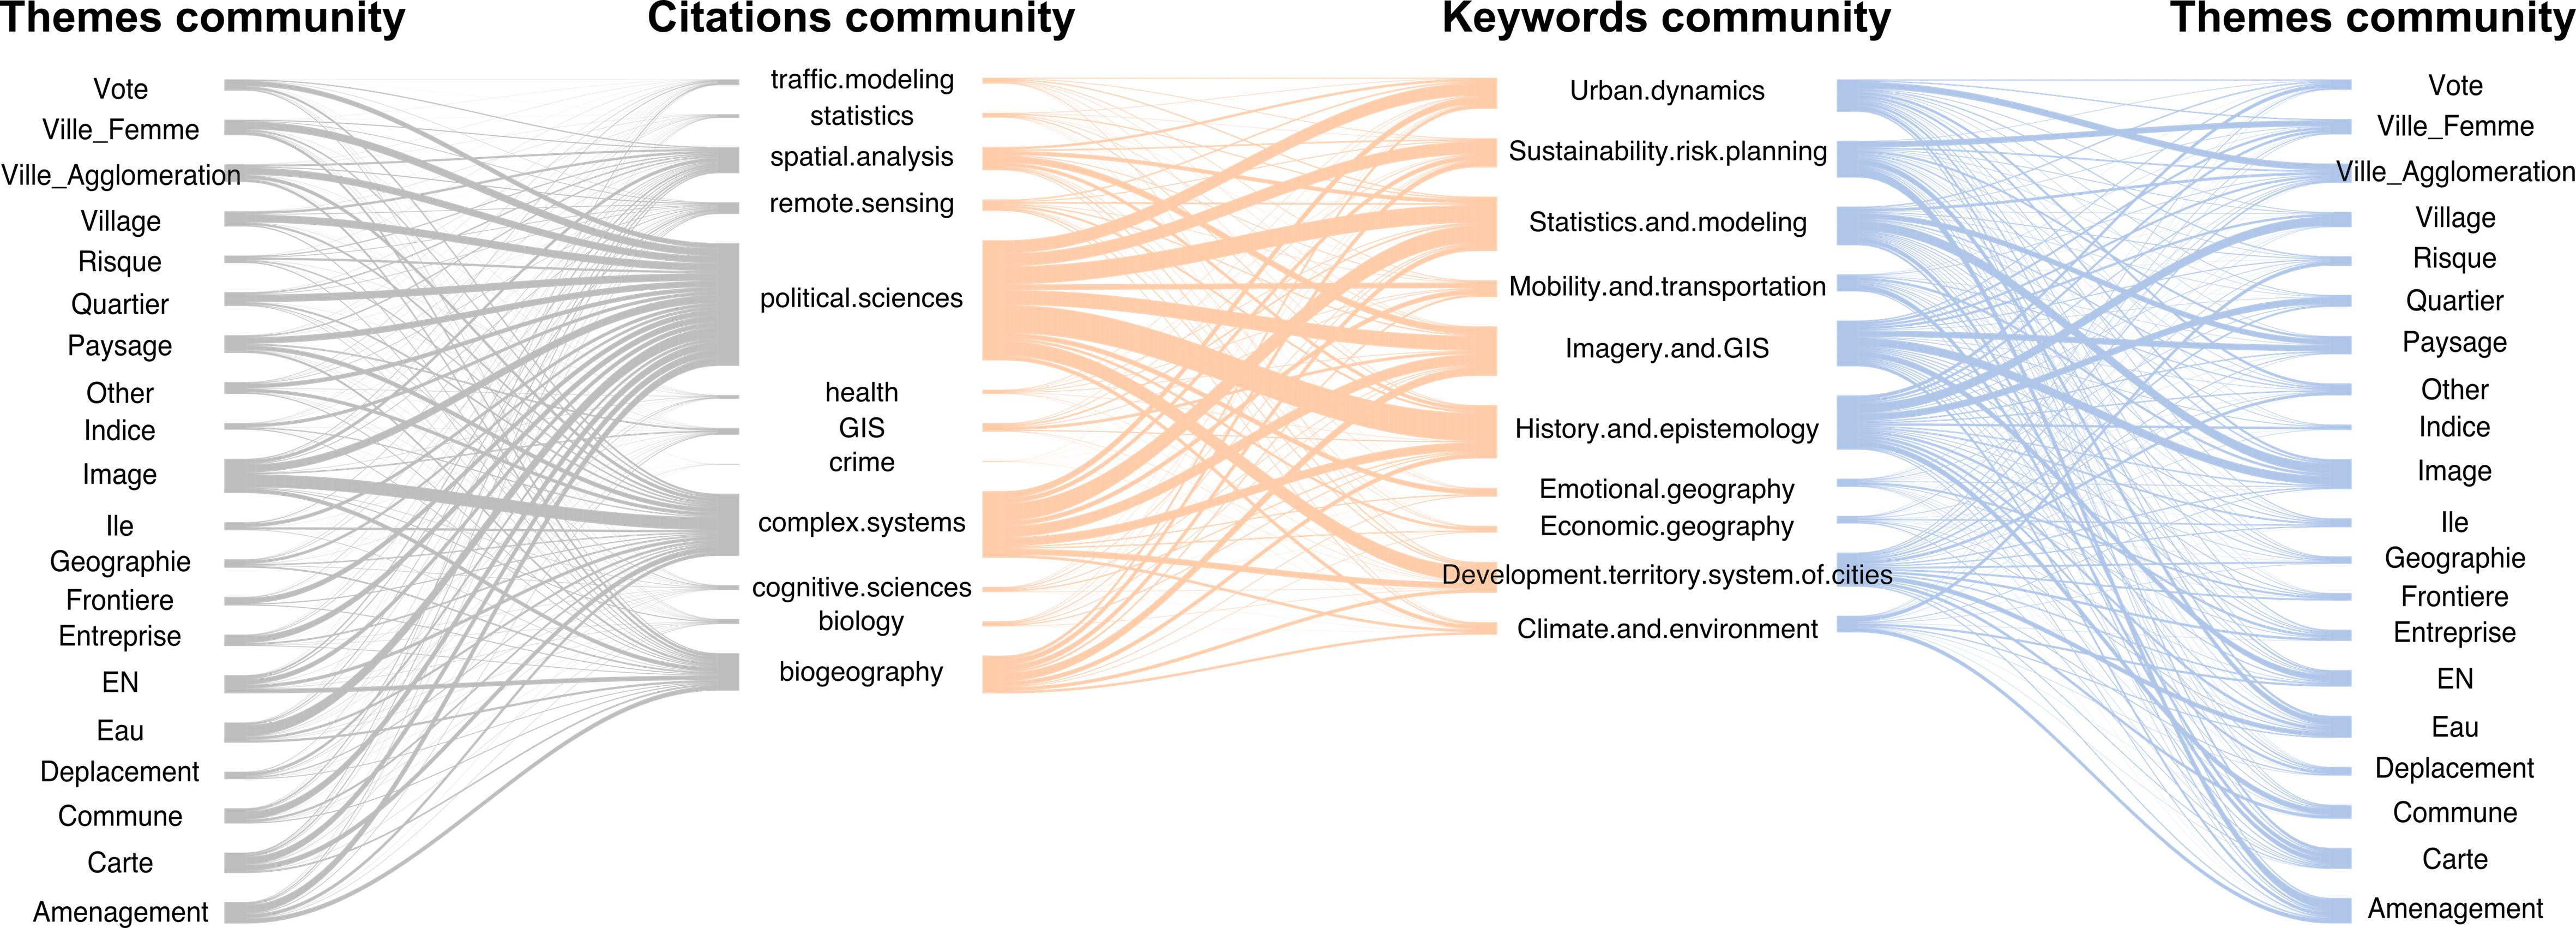
\includegraphics[width=\linewidth]{Figures/CybergeoNetworks/Sankey_methods_Compared.png}
\appcaption{\textbf{Overlap between semantic communities.}\label{fig:app:cybergeonetworks:complementarity}}{\textbf{Recouvrement entre les communautés sémantiques.}\label{fig:app:cybergeonetworks:complementarity}}
\end{figure}
%%%%%%%%%%%%%%%%%%%%%


\bpar{
For instance, there are clear preferential positive and negative relations between some citations communities and keywords communities (figure \ref{fig:complementarity}). On the one hand, 35\% of the Cybergeo articles cited by papers in the GIS cluster are characterized by keywords identified as "Imagery and GIS". On the hand, there is no article cited by papers in the "crime" cluster which have keywords of the "Climate and environment" community. These relationships make sense, because the way a paper is advertised by its keywords is one of the first elements indicating the potential reader that the paper is relevant or not. Interestingly, the "complex systems" citation community is characterized by a variety of keywords communities (27\% of the articles cited by this community are tagged in the "statistics and modelling" cluster, 17\% in "Imagery and GIS" cluster, 13\% in "history and epistemology", 11\% in "urban dynamics"). This suggests that the field of complex systems, being unified by methods rather than objects of inquiry, are more open to diverse topics than other citing communities. It could also mean that within Cybergeo, authors of articles relevant to the complex systems community advertise their paper with keywords from the discipline of geography rather than methods only in order to attract topical reader as well.
}{

}



\bpar{
Looking at the relations between keywords communities and themes communities, we find that some topics require specific words to write about them. For example, "Imagery and GIS"-tagged articles use more words from the "EN" theme category, which corresponds to English words (rather than French). Urban studies are distinguished between its quantitative side (advertised by keywords around "urban dynamics" and using words such as "agglomeration") and its qualitative side (advertised by keywords around "sustainability, risk and planning" and using words such as "\textit{femme}":  woman). Interestingly, the words like "risk" (\textit{risque}) are used themselves more in articles tagged around "Climate and environment" than around "sustainability, risk and planning". Finally, the flows between themes communities and citations communities appear roughly proportional to the size of clusters at origin and destination, suggesting that citations are rather independent of the vocabulary used in the articles. This is reflected in the quantitative analysis below (figure \ref{fig:modularities}), this pair having the smallest mean absolute correlation. In short, the words that count in a citation strategy are much more the keywords than the actual content of the paper.
}{

}


\bpar{
We synthesize the flow relations between classifications by looking at their covariance structure in an aggregated way. More precisely, given the probability matrices $(p_{ki}) = (P_i)$ and $(p_{kj}) = (P_j)$ summarizing two classifications, where articles are indexed by rows, we estimate the correlation matrix between their columns $\rho_{ij} = \hat{\rho}\left[P_i,P_j\right]$ using a standard Pearson correlation estimator. We look then at aggregated measures, namely minimal correlation, maximal correlation and mean absolute correlation. In order to have a reference to interpret the values of these correlations, we compare them to two null models obtained by bootstrapping random corpuses. The estimate for the lower null model ($\rho_0$) is expected to minimize correlation and is obtained by shuffling all rows of one of the two matrices, which is done successively on both to ensure symmetry. The upper null model ($\rho_+$) is constructed by computing correlations between one matrix and the same where a fixed proportion of rows have been shuffled. We set this proportion to 50\%, which is a rather high level of similarity, and compute the model for both matrices each time. Average and standard deviations are computed for null models on $b=10000$ bootstrap repetitions. Table~\ref{tab:cors} summarizes the results. We find that the maximal correlation for the Cybergeo corpus, which can be interpreted as a maximum overlap between approaches of semantic clustering, is always significantly smaller (around $5\cdot \sigma$) than for the upper null model. This confirms that our three classifications are highly independent of one another in their main components. It is interesting to note that for Keywords/Themes, the mean absolute correlation is within the standard error range of the mean absolute correlation of the upper null model, suggesting that these two must be rather close on small overlaps. They are actually closer than with Citations for all indicators. We also confirm that Themes/Citations has the lowest mean absolute overlap.
}{

}


%%%%%%%%%%%%%%
\begin{table}%[htbp]
\begin{threeparttable}
\appcaption{\textbf{Correlations between classifications.}\label{tab:app:cybergeonetworks:cors}}{\textbf{Corrélations entre les classifications.}\label{tab:app:cybergeonetworks:cors}}
\begin{tabular}{lccccccccc}
 \toprule
 \hline\cr
 & $\min \rho$ & $\min \rho_0$ & $\min \rho_+$ & $\max \rho$ & $\max \rho_0$ &$\max \rho_+$ & $< \left| \rho \right|>$ & $< \left| \rho_0 \right|>$ & $< \left| \rho_+ \right|>$ \\\cr\hline\cr
 Themes/Citations & -0.30 &$-0.12$&$-0.17$&0.36&$0.21$&$0.69$&0.059&$0.043$&$0.073$\\
  &  &$\pm 0.019$&$\pm 0.071$&&$\pm 0.042$&$\pm 0.070$&&$\pm 0.0021$&$\pm 0.012$\\\cr
 Citations/Keywords & -0.26 & $-0.096$ & $-0.20$ & 0.30 & $ 0.13$ & $0.64$ & 0.070 & $ 0.034$ & $ 0.092$\\
  &  & $\pm 0.015$ & $\pm 0.047$ && $\pm 0.027 $ & $\pm0.068$ & & $\pm 0.0026 $ & $\pm 0.0081$\\\cr
 Keywords/Themes &-0.20&$-0.11$&$-0.13$&0.51&$0.17$&$0.66$&0.091&$0.040$&$0.080$\\
  &&$\pm0.013$&$\pm0.030$&&$\pm0.032$&$\pm0.075$&&$\pm0.0022$&$\pm0.020$\\\cr
 \hline
\bottomrule
\end{tabular}
 \begin{tablenotes}
       \item \protect\scriptsize{\textbf{Notes}: For each pair of classification and measure, we also give average and standard deviation for lower ($\rho_0$) and upper ($\rho_+$) null models, obtained by bootstrapping $b=10000$ random corpuses.}
    \end{tablenotes}
  \end{threeparttable}
\end{table}
%%%%%%%%%%%%%%



\bpar{
To make these conclusions more robust, we complement the analysis with a network modularity analysis, which is a widely applied method to evaluate the relevance of a classification within a network. To be able to compare two classifications, since the citation network is too sparse for any analysis as mentioned, we evaluate the modularity of a classification within the network induced by the other. More precisely, given a distance threshold $\theta$ and two documents given by their probabilities within a classification $\vec{p}_i^{(c)},\vec{p}_j^{(c)}$, we consider the network with documents as nodes linked if and only if $d(\vec{p}_i^{(c)},\vec{p}_j^{(c)})<\theta$ with $d$ euclidian distance. We can then compute the multi-class modularity of the other classification in the sense of~\cite{nicosia2009extending}. We show in Fig.~\ref{fig:modularities}, for different thresholds, the modularities normalized by the modularity of the network classification within its own network. The closest the measure is to 1, the closer are the classifications. Most of couple have low values for large ranges of $\theta$, confirming the previous conclusions of orthogonality. Furthermore, the different behavior as a function of $\theta$ (increasing or decreasing) suggests different \emph{internal structures} of classification, what is consistent with the fact that they rely on different processes to classify data.
}{

}

%%%%%%%%%%%%%%%%%%%%%
\begin{figure}%[htbp]
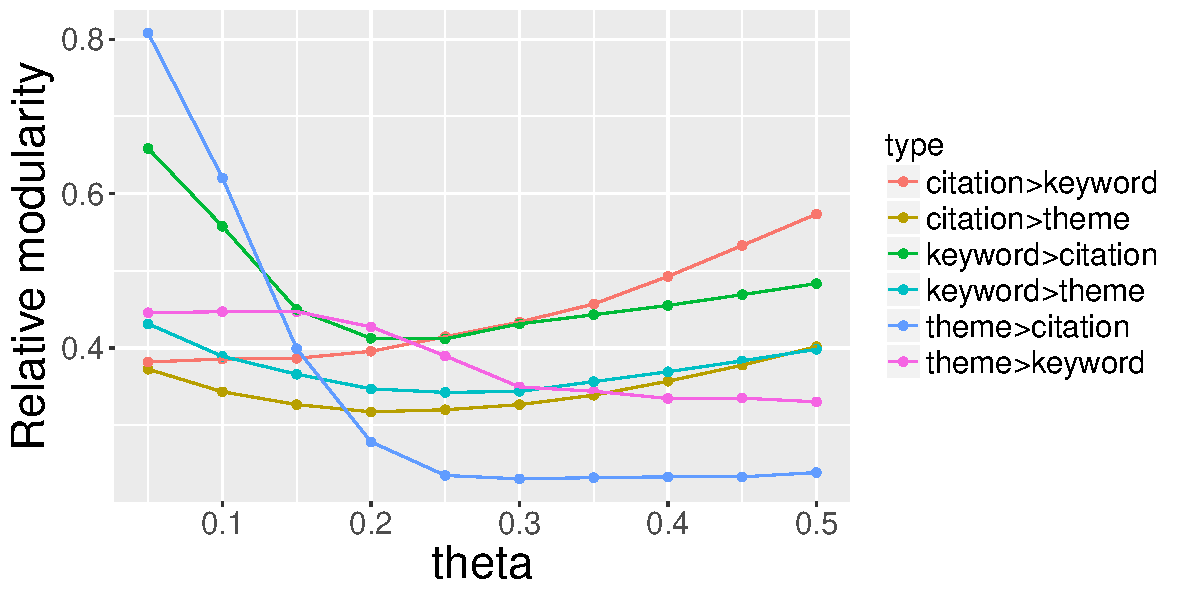
\includegraphics[width=\linewidth]{Figures/CybergeoNetworks/modularities}
\appcaption{\textbf{Evaluating the complementarity of classification through network modularities.} The plot gives the relative modularity of the first classification in the network induced by the second with the threshold $\theta$ (see text), for each couple of classifications (color).\label{fig:app:cybergeonetworks:modularities}}{\textbf{Evaluation de la complémentarité des classifications par la modularités des réseaux.} Le graphe \label{fig:app:cybergeonetworks:modularities}}
\end{figure}
%%%%%%%%%%%%%%%%%%%%%



\bpar{
Together with the visual diagrams, these analyses show the complementarity of classifications in the exploration of semantic diversity of publication in a 20 year old journal.
}{

}


%%%%%%%%%%%%%%%%%%%%%
\subsubsection{Applied Perspectivism}{Perspectivisme appliqué}

\bpar{
Our approach can be understood as an ``applied perspectivism'', which we believe is a way to enhance second order knowledge creation and to ensure reflexivity. Perspectivism is an epistemological position defended by~\cite{giere2010scientific}, that aims at going beyond the constructivism-reductivism debates. Focusing on scientific agents as carriers of knowledge creation, any scientific entreprise is a certain \emph{perspective} on the world, taken by the agent for a given purpose and through a given medium that is considered as the \emph{model}. Perspectives are necessary complementary as they result from different approaches to the same objects, even if the definition of objects and research questions will not necessarily be the same. Coupling perspectives should thus be a typical feature of interdisciplinarity. We position our work as a deliberate attempt to couple complementary perspectives on the same corpus. \cite{varenne2017theories} recalls that one of the various function of models is to foster coupling between theories through coupling of models themselves, allowing the creation of novel knowledge within the virtuous spiral between disciplinarity and interdisciplinarity coined by~\cite{banos2013pour}. Our work aims precisely at accelerating and improving such processes.
}{
Notre approche peut être comprise comme un ``perspectivisme appliqué'', que nous postulons comme une manière de contribuer à la création d'une connaissance au second ordre et d'assurer une réflexivité. Le perspectivisme est une position épistémologique défendue par~\cite{giere2010scientific}, qui vise à sortir par le haut des débats entre constructivisme et réalisme. En se concentrant sur les agents scientifiques comme supports de la création de connaissances, toute entreprise scientifique est une certaine \emph{perspective} sur le monde, prise par l'agent dans un certain but et grâce à un certain medium qui est considéré comme étant son \emph{modèle}. Les perspectives sont généralement complémentaires puisqu'elles résultent d'approches différentes sur les mêmes objets, bien que les définitions des objets et les questions de recherche ne seront pas nécessairement les mêmes. Le couplage de perspectives devrait ainsi être une caractéristique essentielle de l'interdisciplinarité. Nous positionnons notre travail comme une tentative délibérée de coupler des perspectives complémentaires sur le même corpus. \cite{varenne2017theories} rappelle que l'une des nombreuses fonctions des modèles est de favoriser le couplage entre théories par le couplage des modèles eux-mêmes, permettant la création d'une connaissance nouvelle au sein de la spirale vertueuse entre disciplinarité et interdisciplinarité mise en valeur par~\cite{banos2013pour}. Notre travail vise précisément à accélérer et améliorer de tels processus.
}


%%%%%%%%%%%%%%%%%
\subsubsection{Fostering Open Science and Reflexivity}{Encourager la Science ouverte et la Réflexivité}

\bpar{
The open tools and software we provide participate to a larger effort of reflexivity tools in the context of Open Science. It is aimed at being complementary to existing platforms, like the Community Explorer for the community of Complex Systems developed by ISCPIF\footnote{available at \url{https://communityexplorer.org}} that provides an interactive visualisation of social research networks combined to semantic networks based on self-declared keywords provided by researchers. An other example closer to what we developed is Gargantext\footnote{\url{https://gargantext.org/}} that provides corpus exploration functionalities. Linkage\footnote{\url{https://linkage.fr/}} is a similar tool with different methods, using latent topic allocation for networks with textual annotations~\citep{bouveyron2016stochastic}. We differentiate from these by exploring simultaneously multiple dimensions of semantic classification and more importantly by adding the geographical aspect. Furthermore, in comparison to various tools that private publishers are beginning to introduce, the open and collaborative nature of our work is crucial. For example, \cite{bohannon2014google} suggests that one must stay careful when using search results from a popular academic search engine, as the mechanisms of the ranking algorithm and thus the multiple biases are unknown. The comparison is similar with text-mining paying services provided by private companies, as we suggest that a subtle synergy between knowledge content and knowledge production processes (that is allowed by open tools only) can be more beneficial to both.
}{
Les outils ouverts et les logiciels que nous produisons participent à un effort plus large de conception d'outils de réflexivité dans le contexte de la Science Ouverte. Ils visent à être complémentaires aux plateformes existantes, comme le \textit{Community Explorer} développé pour la communauté des Systèmes Complexes développé par l'ISCPIF\footnote{disponible à \url{https://communityexplorer.org}} qui fournit une visualisation interactive des réseaux sociaux de la recherche en combinaison aux réseaux sémantiques basés sur les mots-clés auto-déclarés donnés par les chercheurs. Un autre exemple plus proche de ce que nous avons développé est l'outil Gargantext\footnote{\url{https://gargantext.org/}} qui fournit des fonctions d'exploration de corpus. Linkage\footnote{\url{https://linkage.fr/}} est un outil similaire avec des méthodes différentes, qui utilise un allocation latente de thèmes pour les réseaux avec annotations textuelles~\citep{bouveyron2016stochastic}. Nous nous différentions de ceux-ci en explorant simultanément de multiples dimensions de classification sémantique et de façon plus importante en y ajoutant la composante géographique. De plus, en comparaison aux outils variés que les éditeurs privés commencent à introduire, la nature ouverte et collaborative de notre travail est essentielle. Par exemple, \cite{bohannon2014google} suggère qu'il faut rester précautionneux quant à l'utilisation des résultats de recherche issus d'un engin académique de requêtes populaire, comme les mécanismes de l'algorithme de classement et ainsi les biais multiples restent inconnus. La comparaison est similaire avec les services payant de fouille de texte fournis par des entreprises privées, puisque nous suggérons qu'une synergie subtile entre le contenu de la connaissance et les processus de production de connaissance (qui est permise par des outils ouverts de manière privilégiée) peut être plus bénéfique aux deux.
}




%%%%%%%%%%%%%%%%%%%%%
\subsection{Conclusion}{Conclusion}
%%%%%%%%%%%%%%%%%%%%%


\bpar{
We have studied a scientific corpus of a journal in Geography, combining multiple points of view through their embedding in the geographical space. This work is therefore in itself reflexive, illustrating the kind of new approach to science it aims at promoting. We believe that the open tools we develop in this context will contribute to the empowerment of authors within Open Science.
}{
Nous avons étudié un corpus scientifique d'un journal en Géographie, combinant des points de vue multiples par leur plongement dans l'espace géographique. Ce travail est pour cela en lui-même réflexif, illustrant le type d'approche nouvelle à la science qu'il cherche à promouvoir. Nous sommes convaincus que les outils ouverts que nous développons dans ce contexte contribueront à la prise d'autonomie des auteurs dans la Science Ouverte.
}







